% Kestrel v3 project report. Build: cd paper/v3 && latexmk -pdf kestrel_v3_report.tex
% Every result number is a \kv{key} macro from generated/numbers.tex (experiments/analysis/paper_assets_v3.py, from
% the committed v3 logs). Quoted requests and answers are copied from experiments/logs/v3/acceptance/socket.json.
\documentclass[11pt,a4paper]{article}
\usepackage[margin=2.4cm]{geometry}
\usepackage[T1]{fontenc}
\usepackage{lmodern}
\usepackage{microtype}
\usepackage{amsmath,amssymb}
\usepackage{booktabs}
\usepackage{tabularx}
\usepackage{graphicx}
\usepackage{xcolor}
\usepackage{tikz}
\usetikzlibrary{arrows.meta,positioning,calc,fit}
\usepackage{enumitem}
\usepackage[hidelinks]{hyperref}

\DeclareRobustCommand{\kv}[1]{\ifcsname kv@#1\endcsname\csname kv@#1\endcsname\else\textbf{??#1??}\fi}
% Generated by experiments/analysis/paper_assets_v3.py from the committed logs.
\makeatletter
\expandafter\def\csname kv@e0.gemma.tg\endcsname{\ensuremath{12.1}}
\expandafter\def\csname kv@e0.gemma.pp\endcsname{\ensuremath{58}}
\expandafter\def\csname kv@e0.qsmall.tg\endcsname{\ensuremath{18.2}}
\expandafter\def\csname kv@e0.qsmall.pp\endcsname{\ensuremath{91}}
\expandafter\def\csname kv@e0.qbig.tg\endcsname{\ensuremath{8.2}}
\expandafter\def\csname kv@e0.qbig.pp\endcsname{\ensuremath{36}}
\expandafter\def\csname kv@hw.cpu\endcsname{\ensuremath{Ryzen 5 5500U}}
\expandafter\def\csname kv@hw.cores\endcsname{\ensuremath{6}}
\expandafter\def\csname kv@hw.threads\endcsname{\ensuremath{12}}
\expandafter\def\csname kv@hw.ram\endcsname{\ensuremath{14.95}}
\expandafter\def\csname kv@e1.encoder.median\endcsname{\ensuremath{5.6}}
\expandafter\def\csname kv@kv0.labels\endcsname{\ensuremath{5}}
\expandafter\def\csname kv@kv0.status\endcsname{reviewed}
\expandafter\def\csname kv@kv0.train\endcsname{\ensuremath{820}}
\expandafter\def\csname kv@kv0.cal\endcsname{\ensuremath{103}}
\expandafter\def\csname kv@kv0.val\endcsname{\ensuremath{128}}
\expandafter\def\csname kv@kv0.test\endcsname{\ensuremath{240}}
\expandafter\def\csname kv@kv0.items\endcsname{\ensuremath{1291}}
\expandafter\def\csname kv@kv1.labels\endcsname{\ensuremath{6}}
\expandafter\def\csname kv@kv1.status\endcsname{reviewed}
\expandafter\def\csname kv@kv1.train\endcsname{\ensuremath{920}}
\expandafter\def\csname kv@kv1.cal\endcsname{\ensuremath{115}}
\expandafter\def\csname kv@kv1.val\endcsname{\ensuremath{136}}
\expandafter\def\csname kv@kv1.test\endcsname{\ensuremath{256}}
\expandafter\def\csname kv@kv1.items\endcsname{\ensuremath{1427}}
\expandafter\def\csname kv@kv2.labels\endcsname{\ensuremath{7}}
\expandafter\def\csname kv@kv2.status\endcsname{claude reviewed}
\expandafter\def\csname kv@kv2.train\endcsname{\ensuremath{1000}}
\expandafter\def\csname kv@kv2.train.fresh\endcsname{\ensuremath{80}}
\expandafter\def\csname kv@kv2.cal\endcsname{\ensuremath{123}}
\expandafter\def\csname kv@kv2.cal.fresh\endcsname{\ensuremath{8}}
\expandafter\def\csname kv@kv2.val\endcsname{\ensuremath{152}}
\expandafter\def\csname kv@kv2.val.fresh\endcsname{\ensuremath{16}}
\expandafter\def\csname kv@kv2.test\endcsname{\ensuremath{280}}
\expandafter\def\csname kv@kv2.test.fresh\endcsname{\ensuremath{24}}
\expandafter\def\csname kv@kv2.items\endcsname{\ensuremath{1555}}
\expandafter\def\csname kv@notes.fixture\endcsname{\ensuremath{18}}
\expandafter\def\csname kv@notesq.dev.q\endcsname{\ensuremath{22}}
\expandafter\def\csname kv@notesq.dev.none\endcsname{\ensuremath{4}}
\expandafter\def\csname kv@notesq.dev.fam\endcsname{\ensuremath{11}}
\expandafter\def\csname kv@notesq.dev.found\endcsname{\ensuremath{18}}
\expandafter\def\csname kv@notesq.test.q\endcsname{\ensuremath{20}}
\expandafter\def\csname kv@notesq.test.none\endcsname{\ensuremath{2}}
\expandafter\def\csname kv@notesq.test.fam\endcsname{\ensuremath{10}}
\expandafter\def\csname kv@notesq.test.found\endcsname{\ensuremath{18}}
\expandafter\def\csname kv@notesqa.dev.q\endcsname{\ensuremath{26}}
\expandafter\def\csname kv@notesqa.dev.un\endcsname{\ensuremath{6}}
\expandafter\def\csname kv@notesqa.dev.ans\endcsname{\ensuremath{20}}
\expandafter\def\csname kv@notesqa.dev.fam\endcsname{\ensuremath{12}}
\expandafter\def\csname kv@notesqa.test.q\endcsname{\ensuremath{25}}
\expandafter\def\csname kv@notesqa.test.un\endcsname{\ensuremath{6}}
\expandafter\def\csname kv@notesqa.test.ans\endcsname{\ensuremath{19}}
\expandafter\def\csname kv@notesqa.test.fam\endcsname{\ensuremath{12}}
\expandafter\def\csname kv@code.status\endcsname{claude reviewed}
\expandafter\def\csname kv@code.dev.n\endcsname{\ensuremath{24}}
\expandafter\def\csname kv@code.dev.fam\endcsname{\ensuremath{12}}
\expandafter\def\csname kv@code.dev.pertype\endcsname{\ensuremath{6}}
\expandafter\def\csname kv@code.test.n\endcsname{\ensuremath{24}}
\expandafter\def\csname kv@code.test.fam\endcsname{\ensuremath{12}}
\expandafter\def\csname kv@code.test.pertype\endcsname{\ensuremath{6}}
\expandafter\def\csname kv@kv2.fam.n\endcsname{\ensuremath{32}}
\expandafter\def\csname kv@kv2.fam.app\endcsname{\ensuremath{3}}
\expandafter\def\csname kv@kv2.fam.chat\endcsname{\ensuremath{6}}
\expandafter\def\csname kv@kv2.fam.code\endcsname{\ensuremath{12}}
\expandafter\def\csname kv@kv2.fam.notes\endcsname{\ensuremath{6}}
\expandafter\def\csname kv@kv2.fam.rewrite\endcsname{\ensuremath{5}}
\expandafter\def\csname kv@code.families\endcsname{\ensuremath{24}}
\expandafter\def\csname kv@kh1.c\endcsname{\ensuremath{10}}
\expandafter\def\csname kv@kh1.T\endcsname{\ensuremath{0.67}}
\expandafter\def\csname kv@kh1.folds\endcsname{\ensuremath{5}}
\expandafter\def\csname kv@kh1.oof.acc\endcsname{\ensuremath{0.812}}
\expandafter\def\csname kv@kh1.val.n\endcsname{\ensuremath{136}}
\expandafter\def\csname kv@kh1.val.acc\endcsname{\ensuremath{0.926}}
\expandafter\def\csname kv@kh1.val.f1\endcsname{\ensuremath{0.799}}
\expandafter\def\csname kv@kh1.val.ece.raw\endcsname{\ensuremath{0.147}}
\expandafter\def\csname kv@kh1.val.ece\endcsname{\ensuremath{0.076}}
\expandafter\def\csname kv@fb1.T\endcsname{\ensuremath{1.89}}
\expandafter\def\csname kv@fb1.ms.p50\endcsname{\ensuremath{379}}
\expandafter\def\csname kv@fb1.ms.p95\endcsname{\ensuremath{565}}
\expandafter\def\csname kv@fb1.val.gemma.acc\endcsname{\ensuremath{0.860}}
\expandafter\def\csname kv@fb1.unsure.n\endcsname{\ensuremath{24}}
\expandafter\def\csname kv@fb1.unsure.head\endcsname{\ensuremath{15}}
\expandafter\def\csname kv@fb1.unsure.gemma\endcsname{\ensuremath{18}}
\expandafter\def\csname kv@fb1.tau\endcsname{\ensuremath{0.7}}
\expandafter\def\csname kv@fb1.taug\endcsname{\ensuremath{0.9}}
\expandafter\def\csname kv@fb1.val.right\endcsname{\ensuremath{119/136}}
\expandafter\def\csname kv@kt1.n\endcsname{\ensuremath{256}}
\expandafter\def\csname kv@kt1.head.acc\endcsname{\ensuremath{0.867}}
\expandafter\def\csname kv@kt1.head.f1\endcsname{\ensuremath{0.724}}
\expandafter\def\csname kv@kt1.head.ece\endcsname{\ensuremath{0.025}}
\expandafter\def\csname kv@kt1.gemma.acc\endcsname{\ensuremath{0.820}}
\expandafter\def\csname kv@kt1.ha.right\endcsname{\ensuremath{206/256}}
\expandafter\def\csname kv@kt1.ha.right.pct\endcsname{\ensuremath{80.5\%}}
\expandafter\def\csname kv@kt1.ha.right.ci\endcsname{\ensuremath{[75.2\%, 84.9\%]}}
\expandafter\def\csname kv@kt1.ha.asked\endcsname{\ensuremath{18}}
\expandafter\def\csname kv@kt1.ha.sentoldway\endcsname{\ensuremath{32}}
\expandafter\def\csname kv@kt1.ha.notaskedfor\endcsname{\ensuremath{0}}
\expandafter\def\csname kv@kt1.ha.skill\endcsname{\ensuremath{27/76}}
\expandafter\def\csname kv@kt1.ha.skill.pct\endcsname{\ensuremath{35.5\%}}
\expandafter\def\csname kv@kt1.ha.skill.ci\endcsname{\ensuremath{[25.7\%, 46.7\%]}}
\expandafter\def\csname kv@kt1.ha.app\endcsname{\ensuremath{179/180}}
\expandafter\def\csname kv@kt1.ha.app.pct\endcsname{\ensuremath{99.4\%}}
\expandafter\def\csname kv@kt1.ha.app.ci\endcsname{\ensuremath{[96.9\%, 99.9\%]}}
\expandafter\def\csname kv@kt1.ha.en\endcsname{\ensuremath{107/128}}
\expandafter\def\csname kv@kt1.ha.en.pct\endcsname{\ensuremath{83.6\%}}
\expandafter\def\csname kv@kt1.ha.en.ci\endcsname{\ensuremath{[76.2\%, 89.0\%]}}
\expandafter\def\csname kv@kt1.ha.hi\endcsname{\ensuremath{99/128}}
\expandafter\def\csname kv@kt1.ha.hi.pct\endcsname{\ensuremath{77.3\%}}
\expandafter\def\csname kv@kt1.ha.hi.ci\endcsname{\ensuremath{[69.4\%, 83.7\%]}}
\expandafter\def\csname kv@kt1.ha.kind.app\endcsname{\ensuremath{179/180}}
\expandafter\def\csname kv@kt1.ha.kind.chat\endcsname{\ensuremath{2/16}}
\expandafter\def\csname kv@kt1.ha.kind.email\endcsname{\ensuremath{12/16}}
\expandafter\def\csname kv@kt1.ha.kind.notes\endcsname{\ensuremath{1/12}}
\expandafter\def\csname kv@kt1.ha.kind.rewrite\endcsname{\ensuremath{3/16}}
\expandafter\def\csname kv@kt1.ha.kind.translate\endcsname{\ensuremath{9/16}}
\expandafter\def\csname kv@kt1.hg.right\endcsname{\ensuremath{220/256}}
\expandafter\def\csname kv@kt1.hg.right.pct\endcsname{\ensuremath{85.9\%}}
\expandafter\def\csname kv@kt1.hg.right.ci\endcsname{\ensuremath{[81.1\%, 89.7\%]}}
\expandafter\def\csname kv@kt1.hg.asked\endcsname{\ensuremath{11}}
\expandafter\def\csname kv@kt1.hg.sentoldway\endcsname{\ensuremath{25}}
\expandafter\def\csname kv@kt1.hg.notaskedfor\endcsname{\ensuremath{0}}
\expandafter\def\csname kv@kt1.hg.skill\endcsname{\ensuremath{40/76}}
\expandafter\def\csname kv@kt1.hg.skill.pct\endcsname{\ensuremath{52.6\%}}
\expandafter\def\csname kv@kt1.hg.skill.ci\endcsname{\ensuremath{[41.6\%, 63.5\%]}}
\expandafter\def\csname kv@kt1.hg.app\endcsname{\ensuremath{180/180}}
\expandafter\def\csname kv@kt1.hg.app.pct\endcsname{\ensuremath{100.0\%}}
\expandafter\def\csname kv@kt1.hg.app.ci\endcsname{\ensuremath{[97.9\%, 100.0\%]}}
\expandafter\def\csname kv@kt1.hg.en\endcsname{\ensuremath{113/128}}
\expandafter\def\csname kv@kt1.hg.en.pct\endcsname{\ensuremath{88.3\%}}
\expandafter\def\csname kv@kt1.hg.en.ci\endcsname{\ensuremath{[81.6\%, 92.8\%]}}
\expandafter\def\csname kv@kt1.hg.hi\endcsname{\ensuremath{107/128}}
\expandafter\def\csname kv@kt1.hg.hi.pct\endcsname{\ensuremath{83.6\%}}
\expandafter\def\csname kv@kt1.hg.hi.ci\endcsname{\ensuremath{[76.2\%, 89.0\%]}}
\expandafter\def\csname kv@kt1.hg.kind.app\endcsname{\ensuremath{180/180}}
\expandafter\def\csname kv@kt1.hg.kind.chat\endcsname{\ensuremath{11/16}}
\expandafter\def\csname kv@kt1.hg.kind.email\endcsname{\ensuremath{13/16}}
\expandafter\def\csname kv@kt1.hg.kind.notes\endcsname{\ensuremath{1/12}}
\expandafter\def\csname kv@kt1.hg.kind.rewrite\endcsname{\ensuremath{4/16}}
\expandafter\def\csname kv@kt1.hg.kind.translate\endcsname{\ensuremath{11/16}}
\expandafter\def\csname kv@kt1.head.recall.app\endcsname{\ensuremath{0.99}}
\expandafter\def\csname kv@kt1.head.recall.chat\endcsname{\ensuremath{0.38}}
\expandafter\def\csname kv@kt1.head.recall.email\endcsname{\ensuremath{0.88}}
\expandafter\def\csname kv@kt1.head.recall.notes\endcsname{\ensuremath{0.42}}
\expandafter\def\csname kv@kt1.head.recall.rewrite\endcsname{\ensuremath{0.44}}
\expandafter\def\csname kv@kt1.head.recall.translate\endcsname{\ensuremath{0.69}}
\expandafter\def\csname kv@kh2.c\endcsname{\ensuremath{100}}
\expandafter\def\csname kv@kh2.T\endcsname{\ensuremath{0.93}}
\expandafter\def\csname kv@kh2.folds\endcsname{\ensuremath{5}}
\expandafter\def\csname kv@kh2.oof.acc\endcsname{\ensuremath{0.835}}
\expandafter\def\csname kv@kh2.val.n\endcsname{\ensuremath{152}}
\expandafter\def\csname kv@kh2.val.acc\endcsname{\ensuremath{0.862}}
\expandafter\def\csname kv@kh2.val.f1\endcsname{\ensuremath{0.761}}
\expandafter\def\csname kv@kh2.val.ece.raw\endcsname{\ensuremath{0.059}}
\expandafter\def\csname kv@kh2.val.ece\endcsname{\ensuremath{0.055}}
\expandafter\def\csname kv@fb2.T\endcsname{\ensuremath{1.74}}
\expandafter\def\csname kv@fb2.ms.p50\endcsname{\ensuremath{523}}
\expandafter\def\csname kv@fb2.ms.p95\endcsname{\ensuremath{717}}
\expandafter\def\csname kv@fb2.val.gemma.acc\endcsname{\ensuremath{0.882}}
\expandafter\def\csname kv@fb2.unsure.n\endcsname{\ensuremath{38}}
\expandafter\def\csname kv@fb2.unsure.head\endcsname{\ensuremath{19}}
\expandafter\def\csname kv@fb2.unsure.gemma\endcsname{\ensuremath{30}}
\expandafter\def\csname kv@fb2.tau\endcsname{\ensuremath{0.8}}
\expandafter\def\csname kv@fb2.taug\endcsname{\ensuremath{0.7}}
\expandafter\def\csname kv@fb2.val.right\endcsname{\ensuremath{142/152}}
\expandafter\def\csname kv@kt2.n\endcsname{\ensuremath{280}}
\expandafter\def\csname kv@kt2.head.acc\endcsname{\ensuremath{0.900}}
\expandafter\def\csname kv@kt2.head.f1\endcsname{\ensuremath{0.819}}
\expandafter\def\csname kv@kt2.head.ece\endcsname{\ensuremath{0.072}}
\expandafter\def\csname kv@kt2.gemma.acc\endcsname{\ensuremath{0.864}}
\expandafter\def\csname kv@kt2.ha.right\endcsname{\ensuremath{221/280}}
\expandafter\def\csname kv@kt2.ha.right.pct\endcsname{\ensuremath{78.9\%}}
\expandafter\def\csname kv@kt2.ha.right.ci\endcsname{\ensuremath{[73.8\%, 83.3\%]}}
\expandafter\def\csname kv@kt2.ha.asked\endcsname{\ensuremath{37}}
\expandafter\def\csname kv@kt2.ha.sentoldway\endcsname{\ensuremath{20}}
\expandafter\def\csname kv@kt2.ha.notaskedfor\endcsname{\ensuremath{2}}
\expandafter\def\csname kv@kt2.ha.skill\endcsname{\ensuremath{40/96}}
\expandafter\def\csname kv@kt2.ha.skill.pct\endcsname{\ensuremath{41.7\%}}
\expandafter\def\csname kv@kt2.ha.skill.ci\endcsname{\ensuremath{[32.3\%, 51.7\%]}}
\expandafter\def\csname kv@kt2.ha.app\endcsname{\ensuremath{181/184}}
\expandafter\def\csname kv@kt2.ha.app.pct\endcsname{\ensuremath{98.4\%}}
\expandafter\def\csname kv@kt2.ha.app.ci\endcsname{\ensuremath{[95.3\%, 99.4\%]}}
\expandafter\def\csname kv@kt2.ha.en\endcsname{\ensuremath{114/140}}
\expandafter\def\csname kv@kt2.ha.en.pct\endcsname{\ensuremath{81.4\%}}
\expandafter\def\csname kv@kt2.ha.en.ci\endcsname{\ensuremath{[74.2\%, 87.0\%]}}
\expandafter\def\csname kv@kt2.ha.hi\endcsname{\ensuremath{107/140}}
\expandafter\def\csname kv@kt2.ha.hi.pct\endcsname{\ensuremath{76.4\%}}
\expandafter\def\csname kv@kt2.ha.hi.ci\endcsname{\ensuremath{[68.8\%, 82.7\%]}}
\expandafter\def\csname kv@kt2.ha.kind.app\endcsname{\ensuremath{181/184}}
\expandafter\def\csname kv@kt2.ha.kind.chat\endcsname{\ensuremath{6/20}}
\expandafter\def\csname kv@kt2.ha.kind.code\endcsname{\ensuremath{1/8}}
\expandafter\def\csname kv@kt2.ha.kind.email\endcsname{\ensuremath{12/16}}
\expandafter\def\csname kv@kt2.ha.kind.notes\endcsname{\ensuremath{7/16}}
\expandafter\def\csname kv@kt2.ha.kind.rewrite\endcsname{\ensuremath{6/20}}
\expandafter\def\csname kv@kt2.ha.kind.translate\endcsname{\ensuremath{8/16}}
\expandafter\def\csname kv@kt2.hg.right\endcsname{\ensuremath{256/280}}
\expandafter\def\csname kv@kt2.hg.right.pct\endcsname{\ensuremath{91.4\%}}
\expandafter\def\csname kv@kt2.hg.right.ci\endcsname{\ensuremath{[87.6\%, 94.2\%]}}
\expandafter\def\csname kv@kt2.hg.asked\endcsname{\ensuremath{13}}
\expandafter\def\csname kv@kt2.hg.sentoldway\endcsname{\ensuremath{5}}
\expandafter\def\csname kv@kt2.hg.notaskedfor\endcsname{\ensuremath{6}}
\expandafter\def\csname kv@kt2.hg.skill\endcsname{\ensuremath{78/96}}
\expandafter\def\csname kv@kt2.hg.skill.pct\endcsname{\ensuremath{81.3\%}}
\expandafter\def\csname kv@kt2.hg.skill.ci\endcsname{\ensuremath{[72.3\%, 87.8\%]}}
\expandafter\def\csname kv@kt2.hg.app\endcsname{\ensuremath{178/184}}
\expandafter\def\csname kv@kt2.hg.app.pct\endcsname{\ensuremath{96.7\%}}
\expandafter\def\csname kv@kt2.hg.app.ci\endcsname{\ensuremath{[93.1\%, 98.5\%]}}
\expandafter\def\csname kv@kt2.hg.en\endcsname{\ensuremath{130/140}}
\expandafter\def\csname kv@kt2.hg.en.pct\endcsname{\ensuremath{92.9\%}}
\expandafter\def\csname kv@kt2.hg.en.ci\endcsname{\ensuremath{[87.4\%, 96.1\%]}}
\expandafter\def\csname kv@kt2.hg.hi\endcsname{\ensuremath{126/140}}
\expandafter\def\csname kv@kt2.hg.hi.pct\endcsname{\ensuremath{90.0\%}}
\expandafter\def\csname kv@kt2.hg.hi.ci\endcsname{\ensuremath{[83.9\%, 93.9\%]}}
\expandafter\def\csname kv@kt2.hg.kind.app\endcsname{\ensuremath{178/184}}
\expandafter\def\csname kv@kt2.hg.kind.chat\endcsname{\ensuremath{20/20}}
\expandafter\def\csname kv@kt2.hg.kind.code\endcsname{\ensuremath{7/8}}
\expandafter\def\csname kv@kt2.hg.kind.email\endcsname{\ensuremath{15/16}}
\expandafter\def\csname kv@kt2.hg.kind.notes\endcsname{\ensuremath{12/16}}
\expandafter\def\csname kv@kt2.hg.kind.rewrite\endcsname{\ensuremath{8/20}}
\expandafter\def\csname kv@kt2.hg.kind.translate\endcsname{\ensuremath{16/16}}
\expandafter\def\csname kv@kt2.head.recall.app\endcsname{\ensuremath{0.98}}
\expandafter\def\csname kv@kt2.head.recall.chat\endcsname{\ensuremath{0.50}}
\expandafter\def\csname kv@kt2.head.recall.code\endcsname{\ensuremath{0.63}}
\expandafter\def\csname kv@kt2.head.recall.email\endcsname{\ensuremath{0.88}}
\expandafter\def\csname kv@kt2.head.recall.notes\endcsname{\ensuremath{0.81}}
\expandafter\def\csname kv@kt2.head.recall.rewrite\endcsname{\ensuremath{0.85}}
\expandafter\def\csname kv@kt2.head.recall.translate\endcsname{\ensuremath{0.75}}
\expandafter\def\csname kv@kt2.fresh.ha.right\endcsname{\ensuremath{9/24}}
\expandafter\def\csname kv@kt2.fresh.ha.right.pct\endcsname{\ensuremath{37.5\%}}
\expandafter\def\csname kv@kt2.fresh.ha.right.ci\endcsname{\ensuremath{[21.2\%, 57.3\%]}}
\expandafter\def\csname kv@kt2.fresh.ha.asked\endcsname{\ensuremath{11}}
\expandafter\def\csname kv@kt2.fresh.ha.wrongskill\endcsname{\ensuremath{1}}
\expandafter\def\csname kv@kt2.fresh.hg.right\endcsname{\ensuremath{23/24}}
\expandafter\def\csname kv@kt2.fresh.hg.right.pct\endcsname{\ensuremath{95.8\%}}
\expandafter\def\csname kv@kt2.fresh.hg.right.ci\endcsname{\ensuremath{[79.8\%, 99.3\%]}}
\expandafter\def\csname kv@kt2.fresh.hg.asked\endcsname{\ensuremath{0}}
\expandafter\def\csname kv@kt2.fresh.hg.wrongskill\endcsname{\ensuremath{1}}
\expandafter\def\csname kv@kt2.seen.ha.right\endcsname{\ensuremath{212/256}}
\expandafter\def\csname kv@kt2.seen.ha.right.pct\endcsname{\ensuremath{82.8\%}}
\expandafter\def\csname kv@kt2.seen.ha.right.ci\endcsname{\ensuremath{[77.7\%, 86.9\%]}}
\expandafter\def\csname kv@kt2.seen.ha.asked\endcsname{\ensuremath{26}}
\expandafter\def\csname kv@kt2.seen.ha.wrongskill\endcsname{\ensuremath{1}}
\expandafter\def\csname kv@kt2.seen.hg.right\endcsname{\ensuremath{233/256}}
\expandafter\def\csname kv@kt2.seen.hg.right.pct\endcsname{\ensuremath{91.0\%}}
\expandafter\def\csname kv@kt2.seen.hg.right.ci\endcsname{\ensuremath{[86.9\%, 93.9\%]}}
\expandafter\def\csname kv@kt2.seen.hg.asked\endcsname{\ensuremath{13}}
\expandafter\def\csname kv@kt2.seen.hg.wrongskill\endcsname{\ensuremath{5}}
\expandafter\def\csname kv@md.theta\endcsname{\ensuremath{0.85}}
\expandafter\def\csname kv@md.found\endcsname{\ensuremath{7/18}}
\expandafter\def\csname kv@md.found.pct\endcsname{\ensuremath{38.9\%}}
\expandafter\def\csname kv@md.found.ci\endcsname{\ensuremath{[20.3\%, 61.4\%]}}
\expandafter\def\csname kv@md.noise\endcsname{\ensuremath{0/4}}
\expandafter\def\csname kv@md.rank1\endcsname{\ensuremath{11/18}}
\expandafter\def\csname kv@md.rank1.pct\endcsname{\ensuremath{61.1\%}}
\expandafter\def\csname kv@md.rank1.ci\endcsname{\ensuremath{[38.6\%, 79.7\%]}}
\expandafter\def\csname kv@md.found.en\endcsname{\ensuremath{6/9}}
\expandafter\def\csname kv@md.found.en.pct\endcsname{\ensuremath{66.7\%}}
\expandafter\def\csname kv@md.found.en.ci\endcsname{\ensuremath{[35.4\%, 87.9\%]}}
\expandafter\def\csname kv@md.rank1.en\endcsname{\ensuremath{9/9}}
\expandafter\def\csname kv@md.rank1.en.pct\endcsname{\ensuremath{100.0\%}}
\expandafter\def\csname kv@md.rank1.en.ci\endcsname{\ensuremath{[70.1\%, 100.0\%]}}
\expandafter\def\csname kv@md.found.hi\endcsname{\ensuremath{1/9}}
\expandafter\def\csname kv@md.found.hi.pct\endcsname{\ensuremath{11.1\%}}
\expandafter\def\csname kv@md.found.hi.ci\endcsname{\ensuremath{[2.0\%, 43.5\%]}}
\expandafter\def\csname kv@md.rank1.hi\endcsname{\ensuremath{2/9}}
\expandafter\def\csname kv@md.rank1.hi.pct\endcsname{\ensuremath{22.2\%}}
\expandafter\def\csname kv@md.rank1.hi.ci\endcsname{\ensuremath{[6.3\%, 54.7\%]}}
\expandafter\def\csname kv@md.chunks\endcsname{\ensuremath{52}}
\expandafter\def\csname kv@mdt.theta\endcsname{\ensuremath{0.83}}
\expandafter\def\csname kv@mdt.found\endcsname{\ensuremath{18/18}}
\expandafter\def\csname kv@mdt.found.pct\endcsname{\ensuremath{100.0\%}}
\expandafter\def\csname kv@mdt.found.ci\endcsname{\ensuremath{[82.4\%, 100.0\%]}}
\expandafter\def\csname kv@mdt.noise\endcsname{\ensuremath{0/4}}
\expandafter\def\csname kv@mdt.rank1\endcsname{\ensuremath{18/18}}
\expandafter\def\csname kv@mdt.rank1.pct\endcsname{\ensuremath{100.0\%}}
\expandafter\def\csname kv@mdt.rank1.ci\endcsname{\ensuremath{[82.4\%, 100.0\%]}}
\expandafter\def\csname kv@mdt.found.en\endcsname{\ensuremath{9/9}}
\expandafter\def\csname kv@mdt.found.en.pct\endcsname{\ensuremath{100.0\%}}
\expandafter\def\csname kv@mdt.found.en.ci\endcsname{\ensuremath{[70.1\%, 100.0\%]}}
\expandafter\def\csname kv@mdt.rank1.en\endcsname{\ensuremath{9/9}}
\expandafter\def\csname kv@mdt.rank1.en.pct\endcsname{\ensuremath{100.0\%}}
\expandafter\def\csname kv@mdt.rank1.en.ci\endcsname{\ensuremath{[70.1\%, 100.0\%]}}
\expandafter\def\csname kv@mdt.found.hi\endcsname{\ensuremath{9/9}}
\expandafter\def\csname kv@mdt.found.hi.pct\endcsname{\ensuremath{100.0\%}}
\expandafter\def\csname kv@mdt.found.hi.ci\endcsname{\ensuremath{[70.1\%, 100.0\%]}}
\expandafter\def\csname kv@mdt.rank1.hi\endcsname{\ensuremath{9/9}}
\expandafter\def\csname kv@mdt.rank1.hi.pct\endcsname{\ensuremath{100.0\%}}
\expandafter\def\csname kv@mdt.rank1.hi.ci\endcsname{\ensuremath{[70.1\%, 100.0\%]}}
\expandafter\def\csname kv@mdt.chunks\endcsname{\ensuremath{52}}
\expandafter\def\csname kv@mtt.theta\endcsname{\ensuremath{0.83}}
\expandafter\def\csname kv@mtt.found\endcsname{\ensuremath{14/18}}
\expandafter\def\csname kv@mtt.found.pct\endcsname{\ensuremath{77.8\%}}
\expandafter\def\csname kv@mtt.found.ci\endcsname{\ensuremath{[54.8\%, 91.0\%]}}
\expandafter\def\csname kv@mtt.noise\endcsname{\ensuremath{0/2}}
\expandafter\def\csname kv@mtt.rank1\endcsname{\ensuremath{16/18}}
\expandafter\def\csname kv@mtt.rank1.pct\endcsname{\ensuremath{88.9\%}}
\expandafter\def\csname kv@mtt.rank1.ci\endcsname{\ensuremath{[67.2\%, 96.9\%]}}
\expandafter\def\csname kv@mtt.found.en\endcsname{\ensuremath{7/9}}
\expandafter\def\csname kv@mtt.found.en.pct\endcsname{\ensuremath{77.8\%}}
\expandafter\def\csname kv@mtt.found.en.ci\endcsname{\ensuremath{[45.3\%, 93.7\%]}}
\expandafter\def\csname kv@mtt.rank1.en\endcsname{\ensuremath{8/9}}
\expandafter\def\csname kv@mtt.rank1.en.pct\endcsname{\ensuremath{88.9\%}}
\expandafter\def\csname kv@mtt.rank1.en.ci\endcsname{\ensuremath{[56.5\%, 98.0\%]}}
\expandafter\def\csname kv@mtt.found.hi\endcsname{\ensuremath{7/9}}
\expandafter\def\csname kv@mtt.found.hi.pct\endcsname{\ensuremath{77.8\%}}
\expandafter\def\csname kv@mtt.found.hi.ci\endcsname{\ensuremath{[45.3\%, 93.7\%]}}
\expandafter\def\csname kv@mtt.rank1.hi\endcsname{\ensuremath{8/9}}
\expandafter\def\csname kv@mtt.rank1.hi.pct\endcsname{\ensuremath{88.9\%}}
\expandafter\def\csname kv@mtt.rank1.hi.ci\endcsname{\ensuremath{[56.5\%, 98.0\%]}}
\expandafter\def\csname kv@mtt.chunks\endcsname{\ensuremath{52}}
\expandafter\def\csname kv@qa.dev.ans\endcsname{\ensuremath{20/20}}
\expandafter\def\csname kv@qa.dev.ans.pct\endcsname{\ensuremath{100.0\%}}
\expandafter\def\csname kv@qa.dev.ans.ci\endcsname{\ensuremath{[83.9\%, 100.0\%]}}
\expandafter\def\csname kv@qa.dev.un\endcsname{\ensuremath{4/6}}
\expandafter\def\csname kv@qa.dev.un.pct\endcsname{\ensuremath{66.7\%}}
\expandafter\def\csname kv@qa.dev.un.ci\endcsname{\ensuremath{[30.0\%, 90.3\%]}}
\expandafter\def\csname kv@qa.dev.all\endcsname{\ensuremath{24/26}}
\expandafter\def\csname kv@qa.dev.all.pct\endcsname{\ensuremath{92.3\%}}
\expandafter\def\csname kv@qa.dev.all.ci\endcsname{\ensuremath{[75.9\%, 97.9\%]}}
\expandafter\def\csname kv@qa.dev.s.mean\endcsname{\ensuremath{5.1}}
\expandafter\def\csname kv@qa.dev.s.max\endcsname{\ensuremath{8.8}}
\expandafter\def\csname kv@qa.dev.all.en\endcsname{\ensuremath{11/12}}
\expandafter\def\csname kv@qa.dev.all.en.pct\endcsname{\ensuremath{91.7\%}}
\expandafter\def\csname kv@qa.dev.all.en.ci\endcsname{\ensuremath{[64.6\%, 98.5\%]}}
\expandafter\def\csname kv@qa.dev.all.hi\endcsname{\ensuremath{13/14}}
\expandafter\def\csname kv@qa.dev.all.hi.pct\endcsname{\ensuremath{92.9\%}}
\expandafter\def\csname kv@qa.dev.all.hi.ci\endcsname{\ensuremath{[68.5\%, 98.7\%]}}
\expandafter\def\csname kv@qa.test.ans\endcsname{\ensuremath{19/19}}
\expandafter\def\csname kv@qa.test.ans.pct\endcsname{\ensuremath{100.0\%}}
\expandafter\def\csname kv@qa.test.ans.ci\endcsname{\ensuremath{[83.2\%, 100.0\%]}}
\expandafter\def\csname kv@qa.test.un\endcsname{\ensuremath{6/6}}
\expandafter\def\csname kv@qa.test.un.pct\endcsname{\ensuremath{100.0\%}}
\expandafter\def\csname kv@qa.test.un.ci\endcsname{\ensuremath{[61.0\%, 100.0\%]}}
\expandafter\def\csname kv@qa.test.all\endcsname{\ensuremath{25/25}}
\expandafter\def\csname kv@qa.test.all.pct\endcsname{\ensuremath{100.0\%}}
\expandafter\def\csname kv@qa.test.all.ci\endcsname{\ensuremath{[86.7\%, 100.0\%]}}
\expandafter\def\csname kv@qa.test.s.mean\endcsname{\ensuremath{4.9}}
\expandafter\def\csname kv@qa.test.s.max\endcsname{\ensuremath{6.8}}
\expandafter\def\csname kv@qa.test.all.en\endcsname{\ensuremath{12/12}}
\expandafter\def\csname kv@qa.test.all.en.pct\endcsname{\ensuremath{100.0\%}}
\expandafter\def\csname kv@qa.test.all.en.ci\endcsname{\ensuremath{[75.8\%, 100.0\%]}}
\expandafter\def\csname kv@qa.test.all.hi\endcsname{\ensuremath{13/13}}
\expandafter\def\csname kv@qa.test.all.hi.pct\endcsname{\ensuremath{100.0\%}}
\expandafter\def\csname kv@qa.test.all.hi.ci\endcsname{\ensuremath{[77.2\%, 100.0\%]}}
\expandafter\def\csname kv@qa.dev.hinglish\endcsname{\ensuremath{9/12}}
\expandafter\def\csname kv@qa.dev.hinglish.pct\endcsname{\ensuremath{75.0\%}}
\expandafter\def\csname kv@qa.dev.hinglish.ci\endcsname{\ensuremath{[46.8\%, 91.1\%]}}
\expandafter\def\csname kv@qa.test.hinglish\endcsname{\ensuremath{4/10}}
\expandafter\def\csname kv@qa.test.hinglish.pct\endcsname{\ensuremath{40.0\%}}
\expandafter\def\csname kv@qa.test.hinglish.ci\endcsname{\ensuremath{[16.8\%, 68.7\%]}}
\expandafter\def\csname kv@code.test.all\endcsname{\ensuremath{21/24}}
\expandafter\def\csname kv@code.test.all.pct\endcsname{\ensuremath{87.5\%}}
\expandafter\def\csname kv@code.test.all.ci\endcsname{\ensuremath{[69.0\%, 95.7\%]}}
\expandafter\def\csname kv@code.test.all.p1\endcsname{\ensuremath{21/24}}
\expandafter\def\csname kv@code.test.explain\endcsname{\ensuremath{6/6}}
\expandafter\def\csname kv@code.test.explain.pct\endcsname{\ensuremath{100.0\%}}
\expandafter\def\csname kv@code.test.explain.ci\endcsname{\ensuremath{[61.0\%, 100.0\%]}}
\expandafter\def\csname kv@code.test.explain.p1\endcsname{\ensuremath{6/6}}
\expandafter\def\csname kv@code.test.fix\endcsname{\ensuremath{6/6}}
\expandafter\def\csname kv@code.test.fix.pct\endcsname{\ensuremath{100.0\%}}
\expandafter\def\csname kv@code.test.fix.ci\endcsname{\ensuremath{[61.0\%, 100.0\%]}}
\expandafter\def\csname kv@code.test.fix.p1\endcsname{\ensuremath{6/6}}
\expandafter\def\csname kv@code.test.function\endcsname{\ensuremath{6/6}}
\expandafter\def\csname kv@code.test.function.pct\endcsname{\ensuremath{100.0\%}}
\expandafter\def\csname kv@code.test.function.ci\endcsname{\ensuremath{[61.0\%, 100.0\%]}}
\expandafter\def\csname kv@code.test.function.p1\endcsname{\ensuremath{6/6}}
\expandafter\def\csname kv@code.test.script\endcsname{\ensuremath{3/6}}
\expandafter\def\csname kv@code.test.script.pct\endcsname{\ensuremath{50.0\%}}
\expandafter\def\csname kv@code.test.script.ci\endcsname{\ensuremath{[18.8\%, 81.2\%]}}
\expandafter\def\csname kv@code.test.script.p1\endcsname{\ensuremath{3/6}}
\expandafter\def\csname kv@code.test.en\endcsname{\ensuremath{11/12}}
\expandafter\def\csname kv@code.test.en.pct\endcsname{\ensuremath{91.7\%}}
\expandafter\def\csname kv@code.test.en.ci\endcsname{\ensuremath{[64.6\%, 98.5\%]}}
\expandafter\def\csname kv@code.test.en.p1\endcsname{\ensuremath{11/12}}
\expandafter\def\csname kv@code.test.hi\endcsname{\ensuremath{10/12}}
\expandafter\def\csname kv@code.test.hi.pct\endcsname{\ensuremath{83.3\%}}
\expandafter\def\csname kv@code.test.hi.ci\endcsname{\ensuremath{[55.2\%, 95.3\%]}}
\expandafter\def\csname kv@code.test.hi.p1\endcsname{\ensuremath{10/12}}
\expandafter\def\csname kv@code.test.retries\endcsname{\ensuremath{0}}
\expandafter\def\csname kv@code.test.s\endcsname{\ensuremath{8.9}}
\expandafter\def\csname kv@code.test.loopgain\endcsname{\ensuremath{0}}
\expandafter\def\csname kv@code.test.ms.median\endcsname{\ensuremath{7.4}}
\expandafter\def\csname kv@code.test.s.max\endcsname{\ensuremath{20.1}}
\expandafter\def\csname kv@code.test.explain.hi.hinglish\endcsname{\ensuremath{3/3}}
\expandafter\def\csname kv@code.test.explain.en.english\endcsname{\ensuremath{0/3}}
\expandafter\def\csname kv@code.devfinal.all\endcsname{\ensuremath{23/24}}
\expandafter\def\csname kv@code.devfinal.all.pct\endcsname{\ensuremath{95.8\%}}
\expandafter\def\csname kv@code.devfinal.all.ci\endcsname{\ensuremath{[79.8\%, 99.3\%]}}
\expandafter\def\csname kv@code.devfinal.all.p1\endcsname{\ensuremath{23/24}}
\expandafter\def\csname kv@code.devfinal.explain\endcsname{\ensuremath{6/6}}
\expandafter\def\csname kv@code.devfinal.explain.pct\endcsname{\ensuremath{100.0\%}}
\expandafter\def\csname kv@code.devfinal.explain.ci\endcsname{\ensuremath{[61.0\%, 100.0\%]}}
\expandafter\def\csname kv@code.devfinal.explain.p1\endcsname{\ensuremath{6/6}}
\expandafter\def\csname kv@code.devfinal.fix\endcsname{\ensuremath{6/6}}
\expandafter\def\csname kv@code.devfinal.fix.pct\endcsname{\ensuremath{100.0\%}}
\expandafter\def\csname kv@code.devfinal.fix.ci\endcsname{\ensuremath{[61.0\%, 100.0\%]}}
\expandafter\def\csname kv@code.devfinal.fix.p1\endcsname{\ensuremath{6/6}}
\expandafter\def\csname kv@code.devfinal.function\endcsname{\ensuremath{6/6}}
\expandafter\def\csname kv@code.devfinal.function.pct\endcsname{\ensuremath{100.0\%}}
\expandafter\def\csname kv@code.devfinal.function.ci\endcsname{\ensuremath{[61.0\%, 100.0\%]}}
\expandafter\def\csname kv@code.devfinal.function.p1\endcsname{\ensuremath{6/6}}
\expandafter\def\csname kv@code.devfinal.script\endcsname{\ensuremath{5/6}}
\expandafter\def\csname kv@code.devfinal.script.pct\endcsname{\ensuremath{83.3\%}}
\expandafter\def\csname kv@code.devfinal.script.ci\endcsname{\ensuremath{[43.6\%, 97.0\%]}}
\expandafter\def\csname kv@code.devfinal.script.p1\endcsname{\ensuremath{5/6}}
\expandafter\def\csname kv@code.devfinal.en\endcsname{\ensuremath{12/12}}
\expandafter\def\csname kv@code.devfinal.en.pct\endcsname{\ensuremath{100.0\%}}
\expandafter\def\csname kv@code.devfinal.en.ci\endcsname{\ensuremath{[75.8\%, 100.0\%]}}
\expandafter\def\csname kv@code.devfinal.en.p1\endcsname{\ensuremath{12/12}}
\expandafter\def\csname kv@code.devfinal.hi\endcsname{\ensuremath{11/12}}
\expandafter\def\csname kv@code.devfinal.hi.pct\endcsname{\ensuremath{91.7\%}}
\expandafter\def\csname kv@code.devfinal.hi.ci\endcsname{\ensuremath{[64.6\%, 98.5\%]}}
\expandafter\def\csname kv@code.devfinal.hi.p1\endcsname{\ensuremath{11/12}}
\expandafter\def\csname kv@code.devfinal.retries\endcsname{\ensuremath{0}}
\expandafter\def\csname kv@code.devfinal.s\endcsname{\ensuremath{9.1}}
\expandafter\def\csname kv@code.devfinal.loopgain\endcsname{\ensuremath{0}}
\expandafter\def\csname kv@code.devfinal.ms.median\endcsname{\ensuremath{7.6}}
\expandafter\def\csname kv@code.devfinal.s.max\endcsname{\ensuremath{28.1}}
\expandafter\def\csname kv@code.devfinal.explain.hi.hinglish\endcsname{\ensuremath{3/3}}
\expandafter\def\csname kv@code.devfinal.explain.en.english\endcsname{\ensuremath{0/3}}
\expandafter\def\csname kv@code.dev.gemma.all\endcsname{\ensuremath{19/24}}
\expandafter\def\csname kv@code.dev.gemma.all.pct\endcsname{\ensuremath{79.2\%}}
\expandafter\def\csname kv@code.dev.gemma.all.ci\endcsname{\ensuremath{[59.5\%, 90.8\%]}}
\expandafter\def\csname kv@code.dev.gemma.all.p1\endcsname{\ensuremath{19/24}}
\expandafter\def\csname kv@code.dev.gemma.explain\endcsname{\ensuremath{6/6}}
\expandafter\def\csname kv@code.dev.gemma.explain.pct\endcsname{\ensuremath{100.0\%}}
\expandafter\def\csname kv@code.dev.gemma.explain.ci\endcsname{\ensuremath{[61.0\%, 100.0\%]}}
\expandafter\def\csname kv@code.dev.gemma.explain.p1\endcsname{\ensuremath{6/6}}
\expandafter\def\csname kv@code.dev.gemma.fix\endcsname{\ensuremath{6/6}}
\expandafter\def\csname kv@code.dev.gemma.fix.pct\endcsname{\ensuremath{100.0\%}}
\expandafter\def\csname kv@code.dev.gemma.fix.ci\endcsname{\ensuremath{[61.0\%, 100.0\%]}}
\expandafter\def\csname kv@code.dev.gemma.fix.p1\endcsname{\ensuremath{6/6}}
\expandafter\def\csname kv@code.dev.gemma.function\endcsname{\ensuremath{6/6}}
\expandafter\def\csname kv@code.dev.gemma.function.pct\endcsname{\ensuremath{100.0\%}}
\expandafter\def\csname kv@code.dev.gemma.function.ci\endcsname{\ensuremath{[61.0\%, 100.0\%]}}
\expandafter\def\csname kv@code.dev.gemma.function.p1\endcsname{\ensuremath{6/6}}
\expandafter\def\csname kv@code.dev.gemma.script\endcsname{\ensuremath{1/6}}
\expandafter\def\csname kv@code.dev.gemma.script.pct\endcsname{\ensuremath{16.7\%}}
\expandafter\def\csname kv@code.dev.gemma.script.ci\endcsname{\ensuremath{[3.0\%, 56.4\%]}}
\expandafter\def\csname kv@code.dev.gemma.script.p1\endcsname{\ensuremath{1/6}}
\expandafter\def\csname kv@code.dev.gemma.en\endcsname{\ensuremath{10/12}}
\expandafter\def\csname kv@code.dev.gemma.en.pct\endcsname{\ensuremath{83.3\%}}
\expandafter\def\csname kv@code.dev.gemma.en.ci\endcsname{\ensuremath{[55.2\%, 95.3\%]}}
\expandafter\def\csname kv@code.dev.gemma.en.p1\endcsname{\ensuremath{10/12}}
\expandafter\def\csname kv@code.dev.gemma.hi\endcsname{\ensuremath{9/12}}
\expandafter\def\csname kv@code.dev.gemma.hi.pct\endcsname{\ensuremath{75.0\%}}
\expandafter\def\csname kv@code.dev.gemma.hi.ci\endcsname{\ensuremath{[46.8\%, 91.1\%]}}
\expandafter\def\csname kv@code.dev.gemma.hi.p1\endcsname{\ensuremath{9/12}}
\expandafter\def\csname kv@code.dev.gemma.retries\endcsname{\ensuremath{0}}
\expandafter\def\csname kv@code.dev.gemma.s\endcsname{\ensuremath{11.1}}
\expandafter\def\csname kv@code.dev.gemma.loopgain\endcsname{\ensuremath{0}}
\expandafter\def\csname kv@code.dev.gemma.ms.median\endcsname{\ensuremath{10.8}}
\expandafter\def\csname kv@code.dev.gemma.s.max\endcsname{\ensuremath{21.8}}
\expandafter\def\csname kv@code.dev.gemma.explain.hi.hinglish\endcsname{\ensuremath{3/3}}
\expandafter\def\csname kv@code.dev.gemma.explain.en.english\endcsname{\ensuremath{0/3}}
\expandafter\def\csname kv@code.dev.qsmall.all\endcsname{\ensuremath{17/24}}
\expandafter\def\csname kv@code.dev.qsmall.all.pct\endcsname{\ensuremath{70.8\%}}
\expandafter\def\csname kv@code.dev.qsmall.all.ci\endcsname{\ensuremath{[50.8\%, 85.1\%]}}
\expandafter\def\csname kv@code.dev.qsmall.all.p1\endcsname{\ensuremath{17/24}}
\expandafter\def\csname kv@code.dev.qsmall.explain\endcsname{\ensuremath{6/6}}
\expandafter\def\csname kv@code.dev.qsmall.explain.pct\endcsname{\ensuremath{100.0\%}}
\expandafter\def\csname kv@code.dev.qsmall.explain.ci\endcsname{\ensuremath{[61.0\%, 100.0\%]}}
\expandafter\def\csname kv@code.dev.qsmall.explain.p1\endcsname{\ensuremath{6/6}}
\expandafter\def\csname kv@code.dev.qsmall.fix\endcsname{\ensuremath{5/6}}
\expandafter\def\csname kv@code.dev.qsmall.fix.pct\endcsname{\ensuremath{83.3\%}}
\expandafter\def\csname kv@code.dev.qsmall.fix.ci\endcsname{\ensuremath{[43.6\%, 97.0\%]}}
\expandafter\def\csname kv@code.dev.qsmall.fix.p1\endcsname{\ensuremath{5/6}}
\expandafter\def\csname kv@code.dev.qsmall.function\endcsname{\ensuremath{5/6}}
\expandafter\def\csname kv@code.dev.qsmall.function.pct\endcsname{\ensuremath{83.3\%}}
\expandafter\def\csname kv@code.dev.qsmall.function.ci\endcsname{\ensuremath{[43.6\%, 97.0\%]}}
\expandafter\def\csname kv@code.dev.qsmall.function.p1\endcsname{\ensuremath{5/6}}
\expandafter\def\csname kv@code.dev.qsmall.script\endcsname{\ensuremath{1/6}}
\expandafter\def\csname kv@code.dev.qsmall.script.pct\endcsname{\ensuremath{16.7\%}}
\expandafter\def\csname kv@code.dev.qsmall.script.ci\endcsname{\ensuremath{[3.0\%, 56.4\%]}}
\expandafter\def\csname kv@code.dev.qsmall.script.p1\endcsname{\ensuremath{1/6}}
\expandafter\def\csname kv@code.dev.qsmall.en\endcsname{\ensuremath{10/12}}
\expandafter\def\csname kv@code.dev.qsmall.en.pct\endcsname{\ensuremath{83.3\%}}
\expandafter\def\csname kv@code.dev.qsmall.en.ci\endcsname{\ensuremath{[55.2\%, 95.3\%]}}
\expandafter\def\csname kv@code.dev.qsmall.en.p1\endcsname{\ensuremath{10/12}}
\expandafter\def\csname kv@code.dev.qsmall.hi\endcsname{\ensuremath{7/12}}
\expandafter\def\csname kv@code.dev.qsmall.hi.pct\endcsname{\ensuremath{58.3\%}}
\expandafter\def\csname kv@code.dev.qsmall.hi.ci\endcsname{\ensuremath{[32.0\%, 80.7\%]}}
\expandafter\def\csname kv@code.dev.qsmall.hi.p1\endcsname{\ensuremath{7/12}}
\expandafter\def\csname kv@code.dev.qsmall.retries\endcsname{\ensuremath{0}}
\expandafter\def\csname kv@code.dev.qsmall.s\endcsname{\ensuremath{10.4}}
\expandafter\def\csname kv@code.dev.qsmall.loopgain\endcsname{\ensuremath{0}}
\expandafter\def\csname kv@code.dev.qsmall.ms.median\endcsname{\ensuremath{8.7}}
\expandafter\def\csname kv@code.dev.qsmall.s.max\endcsname{\ensuremath{31.6}}
\expandafter\def\csname kv@code.dev.qsmall.explain.hi.hinglish\endcsname{\ensuremath{1/3}}
\expandafter\def\csname kv@code.dev.qsmall.explain.en.english\endcsname{\ensuremath{3/3}}
\expandafter\def\csname kv@code.dev.qbig.all\endcsname{\ensuremath{23/24}}
\expandafter\def\csname kv@code.dev.qbig.all.pct\endcsname{\ensuremath{95.8\%}}
\expandafter\def\csname kv@code.dev.qbig.all.ci\endcsname{\ensuremath{[79.8\%, 99.3\%]}}
\expandafter\def\csname kv@code.dev.qbig.all.p1\endcsname{\ensuremath{23/24}}
\expandafter\def\csname kv@code.dev.qbig.explain\endcsname{\ensuremath{6/6}}
\expandafter\def\csname kv@code.dev.qbig.explain.pct\endcsname{\ensuremath{100.0\%}}
\expandafter\def\csname kv@code.dev.qbig.explain.ci\endcsname{\ensuremath{[61.0\%, 100.0\%]}}
\expandafter\def\csname kv@code.dev.qbig.explain.p1\endcsname{\ensuremath{6/6}}
\expandafter\def\csname kv@code.dev.qbig.fix\endcsname{\ensuremath{6/6}}
\expandafter\def\csname kv@code.dev.qbig.fix.pct\endcsname{\ensuremath{100.0\%}}
\expandafter\def\csname kv@code.dev.qbig.fix.ci\endcsname{\ensuremath{[61.0\%, 100.0\%]}}
\expandafter\def\csname kv@code.dev.qbig.fix.p1\endcsname{\ensuremath{6/6}}
\expandafter\def\csname kv@code.dev.qbig.function\endcsname{\ensuremath{6/6}}
\expandafter\def\csname kv@code.dev.qbig.function.pct\endcsname{\ensuremath{100.0\%}}
\expandafter\def\csname kv@code.dev.qbig.function.ci\endcsname{\ensuremath{[61.0\%, 100.0\%]}}
\expandafter\def\csname kv@code.dev.qbig.function.p1\endcsname{\ensuremath{6/6}}
\expandafter\def\csname kv@code.dev.qbig.script\endcsname{\ensuremath{5/6}}
\expandafter\def\csname kv@code.dev.qbig.script.pct\endcsname{\ensuremath{83.3\%}}
\expandafter\def\csname kv@code.dev.qbig.script.ci\endcsname{\ensuremath{[43.6\%, 97.0\%]}}
\expandafter\def\csname kv@code.dev.qbig.script.p1\endcsname{\ensuremath{5/6}}
\expandafter\def\csname kv@code.dev.qbig.en\endcsname{\ensuremath{12/12}}
\expandafter\def\csname kv@code.dev.qbig.en.pct\endcsname{\ensuremath{100.0\%}}
\expandafter\def\csname kv@code.dev.qbig.en.ci\endcsname{\ensuremath{[75.8\%, 100.0\%]}}
\expandafter\def\csname kv@code.dev.qbig.en.p1\endcsname{\ensuremath{12/12}}
\expandafter\def\csname kv@code.dev.qbig.hi\endcsname{\ensuremath{11/12}}
\expandafter\def\csname kv@code.dev.qbig.hi.pct\endcsname{\ensuremath{91.7\%}}
\expandafter\def\csname kv@code.dev.qbig.hi.ci\endcsname{\ensuremath{[64.6\%, 98.5\%]}}
\expandafter\def\csname kv@code.dev.qbig.hi.p1\endcsname{\ensuremath{11/12}}
\expandafter\def\csname kv@code.dev.qbig.retries\endcsname{\ensuremath{8}}
\expandafter\def\csname kv@code.dev.qbig.s\endcsname{\ensuremath{29.0}}
\expandafter\def\csname kv@code.dev.qbig.loopgain\endcsname{\ensuremath{0}}
\expandafter\def\csname kv@code.dev.qbig.ms.median\endcsname{\ensuremath{21.6}}
\expandafter\def\csname kv@code.dev.qbig.s.max\endcsname{\ensuremath{83.8}}
\expandafter\def\csname kv@code.dev.qbig.explain.hi.hinglish\endcsname{\ensuremath{0/3}}
\expandafter\def\csname kv@code.dev.qbig.explain.en.english\endcsname{\ensuremath{3/3}}
\expandafter\def\csname kv@code.resc.gemma\endcsname{\ensuremath{22/24}}
\expandafter\def\csname kv@code.resc.gemma.writefix\endcsname{\ensuremath{16/18}}
\expandafter\def\csname kv@code.resc.gemma.script\endcsname{\ensuremath{4/6}}
\expandafter\def\csname kv@code.resc.gemma.s\endcsname{\ensuremath{11.1}}
\expandafter\def\csname kv@code.resc.qsmall\endcsname{\ensuremath{18/24}}
\expandafter\def\csname kv@code.resc.qsmall.writefix\endcsname{\ensuremath{13/18}}
\expandafter\def\csname kv@code.resc.qsmall.script\endcsname{\ensuremath{3/6}}
\expandafter\def\csname kv@code.resc.qsmall.s\endcsname{\ensuremath{10.4}}
\expandafter\def\csname kv@code.resc.qbig\endcsname{\ensuremath{22/24}}
\expandafter\def\csname kv@code.resc.qbig.writefix\endcsname{\ensuremath{17/18}}
\expandafter\def\csname kv@code.resc.qbig.script\endcsname{\ensuremath{5/6}}
\expandafter\def\csname kv@code.resc.qbig.s\endcsname{\ensuremath{29.0}}
\expandafter\def\csname kv@writer.baseline\endcsname{\ensuremath{14/23}}
\expandafter\def\csname kv@writer.n\endcsname{\ensuremath{23}}
\expandafter\def\csname kv@writer.baseline.rewrite-hinglish\endcsname{\ensuremath{2/6}}
\expandafter\def\csname kv@writer.baseline.rewrite-english\endcsname{\ensuremath{5/5}}
\expandafter\def\csname kv@writer.baseline.translate-hindi\endcsname{\ensuremath{0/4}}
\expandafter\def\csname kv@writer.baseline.translate-hinglish\endcsname{\ensuremath{3/4}}
\expandafter\def\csname kv@writer.baseline.translate-english\endcsname{\ensuremath{4/4}}
\expandafter\def\csname kv@writer.final\endcsname{\ensuremath{19/23}}
\expandafter\def\csname kv@writer.final.rewrite-hinglish\endcsname{\ensuremath{5/6}}
\expandafter\def\csname kv@writer.final.rewrite-english\endcsname{\ensuremath{5/5}}
\expandafter\def\csname kv@writer.final.translate-hindi\endcsname{\ensuremath{4/4}}
\expandafter\def\csname kv@writer.final.translate-hinglish\endcsname{\ensuremath{1/4}}
\expandafter\def\csname kv@writer.final.translate-english\endcsname{\ensuremath{4/4}}
\expandafter\def\csname kv@mmap.copy.cold.load\endcsname{\ensuremath{3656}}
\expandafter\def\csname kv@mmap.copy.cold.first\endcsname{\ensuremath{111}}
\expandafter\def\csname kv@mmap.copy.cold.tps\endcsname{\ensuremath{12.0}}
\expandafter\def\csname kv@mmap.copy.cold.anon\endcsname{\ensuremath{3247}}
\expandafter\def\csname kv@mmap.copy.cold.file\endcsname{\ensuremath{8}}
\expandafter\def\csname kv@mmap.map.cold.load\endcsname{\ensuremath{2477}}
\expandafter\def\csname kv@mmap.map.cold.first\endcsname{\ensuremath{111}}
\expandafter\def\csname kv@mmap.map.cold.tps\endcsname{\ensuremath{12.0}}
\expandafter\def\csname kv@mmap.map.cold.anon\endcsname{\ensuremath{1144}}
\expandafter\def\csname kv@mmap.map.cold.file\endcsname{\ensuremath{2702}}
\expandafter\def\csname kv@mmap.copy.warm.load\endcsname{\ensuremath{2596}}
\expandafter\def\csname kv@mmap.copy.warm.first\endcsname{\ensuremath{103}}
\expandafter\def\csname kv@mmap.copy.warm.tps\endcsname{\ensuremath{12.0}}
\expandafter\def\csname kv@mmap.copy.warm.anon\endcsname{\ensuremath{3247}}
\expandafter\def\csname kv@mmap.copy.warm.file\endcsname{\ensuremath{8}}
\expandafter\def\csname kv@mmap.map.warm.load\endcsname{\ensuremath{1383}}
\expandafter\def\csname kv@mmap.map.warm.first\endcsname{\ensuremath{117}}
\expandafter\def\csname kv@mmap.map.warm.tps\endcsname{\ensuremath{12.0}}
\expandafter\def\csname kv@mmap.map.warm.anon\endcsname{\ensuremath{1144}}
\expandafter\def\csname kv@mmap.map.warm.file\endcsname{\ensuremath{2702}}
\expandafter\def\csname kv@mmap.anon.saved\endcsname{\ensuremath{2103}}
\expandafter\def\csname kv@mmap.anon.cut\endcsname{\ensuremath{64.8\%}}
\expandafter\def\csname kv@mmap.first.min\endcsname{\ensuremath{103}}
\expandafter\def\csname kv@mmap.first.max\endcsname{\ensuremath{117}}
\expandafter\def\csname kv@worker.v2.n\endcsname{\ensuremath{3}}
\expandafter\def\csname kv@worker.v2.s\endcsname{\ensuremath{19.1}}
\expandafter\def\csname kv@worker.v2.min\endcsname{\ensuremath{18.0}}
\expandafter\def\csname kv@worker.v2.max\endcsname{\ensuremath{19.3}}
\expandafter\def\csname kv@worker.miss.n\endcsname{\ensuremath{3}}
\expandafter\def\csname kv@worker.miss.s\endcsname{\ensuremath{17.4}}
\expandafter\def\csname kv@worker.miss.min\endcsname{\ensuremath{17.3}}
\expandafter\def\csname kv@worker.miss.max\endcsname{\ensuremath{17.9}}
\expandafter\def\csname kv@worker.hit.n\endcsname{\ensuremath{3}}
\expandafter\def\csname kv@worker.hit.s\endcsname{\ensuremath{2.0}}
\expandafter\def\csname kv@worker.hit.min\endcsname{\ensuremath{2.0}}
\expandafter\def\csname kv@worker.hit.max\endcsname{\ensuremath{2.0}}
\expandafter\def\csname kv@worker.prefix.tokens\endcsname{\ensuremath{1132}}
\expandafter\def\csname kv@worker.v2.anon\endcsname{\ensuremath{3356}}
\expandafter\def\csname kv@worker.hit.anon\endcsname{\ensuremath{1135}}
\expandafter\def\csname kv@worker.speedup\endcsname{\ensuremath{9.5}}
\expandafter\def\csname kv@acc.socket\endcsname{\ensuremath{34/36}}
\expandafter\def\csname kv@acc.socket.pct\endcsname{\ensuremath{94.4\%}}
\expandafter\def\csname kv@acc.socket.ci\endcsname{\ensuremath{[81.9\%, 98.5\%]}}
\expandafter\def\csname kv@acc.socket.failed\endcsname{\ensuremath{2}}
\expandafter\def\csname kv@acc.socket.minutes\endcsname{\ensuremath{3.3}}
\expandafter\def\csname kv@acc.run1\endcsname{\ensuremath{31/35}}
\expandafter\def\csname kv@acc.page.headless\endcsname{\ensuremath{8/8}}
\expandafter\def\csname kv@acc.page.headed\endcsname{\ensuremath{8/8}}
\expandafter\def\csname kv@acc.s.task\endcsname{\ensuremath{0.3}}
\expandafter\def\csname kv@acc.s.taskhi\endcsname{\ensuremath{4.8}}
\expandafter\def\csname kv@acc.s.search\endcsname{\ensuremath{0.3}}
\expandafter\def\csname kv@acc.s.meaning\endcsname{\ensuremath{0.3}}
\expandafter\def\csname kv@acc.s.meaninghi\endcsname{\ensuremath{2.6}}
\expandafter\def\csname kv@acc.s.summary\endcsname{\ensuremath{7.9}}
\expandafter\def\csname kv@acc.s.chat\endcsname{\ensuremath{23.2}}
\expandafter\def\csname kv@acc.s.poem\endcsname{\ensuremath{10.3}}
\expandafter\def\csname kv@acc.s.emailhi\endcsname{\ensuremath{8.5}}
\expandafter\def\csname kv@acc.s.email\endcsname{\ensuremath{10.8}}
\expandafter\def\csname kv@acc.s.rewrite\endcsname{\ensuremath{3.6}}
\expandafter\def\csname kv@acc.s.tohindi\endcsname{\ensuremath{2.8}}
\expandafter\def\csname kv@acc.s.toenglish\endcsname{\ensuremath{3.2}}
\expandafter\def\csname kv@acc.s.qa\endcsname{\ensuremath{9.4}}
\expandafter\def\csname kv@acc.s.qanone\endcsname{\ensuremath{3.0}}
\expandafter\def\csname kv@acc.s.codefn\endcsname{\ensuremath{14.0}}
\expandafter\def\csname kv@acc.s.codefix\endcsname{\ensuremath{4.3}}
\expandafter\def\csname kv@acc.s.explain\endcsname{\ensuremath{19.8}}
\expandafter\def\csname kv@acc.s.essay\endcsname{\ensuremath{58.3}}
\expandafter\def\csname kv@acc.fast\endcsname{\ensuremath{17/36}}
\expandafter\def\csname kv@acc.fast.pct\endcsname{\ensuremath{47.2\%}}
\expandafter\def\csname kv@acc.fast.ci\endcsname{\ensuremath{[32.0\%, 63.0\%]}}
\expandafter\def\csname kv@acc.fast.median\endcsname{\ensuremath{0.3}}
\expandafter\def\csname kv@acc.cargo\endcsname{\ensuremath{448}}
\expandafter\def\csname kv@acc.pytest\endcsname{\ensuremath{510}}
\expandafter\def\csname kv@acc.bwrap\endcsname{\ensuremath{6}}
\expandafter\def\csname kv@acc.worker\endcsname{\ensuremath{4}}
\expandafter\def\csname kv@acc.reminder.due\endcsname{\ensuremath{17{:}31}}
\expandafter\def\csname kv@acc.reminder.made\endcsname{\ensuremath{17{:}29{:}29}}
\expandafter\def\csname kv@acc.reminder.rang\endcsname{\ensuremath{17{:}31{:}02}}
\expandafter\def\csname kv@acc.reminder.late\endcsname{\ensuremath{2}}
\expandafter\def\csname kv@acc.limits\endcsname{\ensuremath{12}}
\makeatother

\newcommand{\ms}{\,ms}
\newcommand{\s}{\,s}
\newcommand{\MiB}{\,MiB}
\definecolor{kestrel}{HTML}{D9692E}
\newcommand{\req}[1]{\textit{``#1''}}
\newcommand{\ans}[1]{\texttt{\small #1}}
\setlist{itemsep=2pt, topsep=4pt}
\setlength{\emergencystretch}{3em}

\begin{document}

\begin{titlepage}
\centering
\vspace*{3cm}
{\Huge\bfseries Kestrel v3\par}
\vspace{6pt}
{\Large An offline personal assistant on a laptop\par}
\vspace{1.2cm}
{\large Project report\par}
\vspace{2cm}
\begin{minipage}{0.78\textwidth}\centering
Kestrel answers in English and Hinglish, keeps tasks and reminders, finds and answers from the user's notes, writes
emails, rewrites and translates text, chats, and writes small Python programs that it checks in a sandbox. All of it
runs on one laptop, without the internet and at no cost.
\end{minipage}
\vfill
{\large [Author name] \\ {[Affiliation]}\par}
\vspace{6pt}
28 October 2026 \quad·\quad version tag \texttt{v3-frozen}
\end{titlepage}

\tableofcontents
\newpage

% ---------------------------------------------------------------------------------------------------------------
\section{Summary}

Kestrel is a personal assistant whose every step runs on the user's own laptop. Version~1 (v1) was a research system
that sorted requests into nine intents: eight app actions (search, open or summarize notes, add or delete a task, a
preference, what it remembers, small talk) and \emph{unsupported}, which it refused. Version~2 made it usable every day: tasks with times, reminders, an always-on service and a
browser page. Version~3 (v3), reported here, set out to make Kestrel answer the requests it used to refuse, on the same
laptop and still completely offline:

\begin{itemize}
  \item tasks and reminders (from v2), in English and Hinglish;
  \item finding notes by meaning, not only by their words, and summarizing them;
  \item answering questions from the user's notes, and saying so when the notes do not answer;
  \item drafting emails, rewriting and translating text, and normal chat;
  \item writing and fixing small Python programs, checked in a sealed sandbox, and explaining code.
\end{itemize}

All of it runs on the CPU of a \kv{hw.cores}-core laptop with \kv{hw.ram}~GiB of memory, with two
models already used in v1: a small multilingual sentence encoder and the 4-bit Gemma-4-E2B language model.
Table~\ref{tab:headline} gives the main results; each comes from a log in the repository.

\begin{table}[h]
\centering\small
\caption{Main results of v3. Test splits were run once, after every setting had been chosen on development data. All
evaluation sets are small and synthetic (written for this project, not by real users).}
\label{tab:headline}
\begin{tabularx}{\textwidth}{Xr}
\toprule
What was measured & Result \\
\midrule
Choosing what kind of answer a request needs (test, $n=\kv{kt2.n}$) & \kv{kt2.hg.right} right \\
\quad \ldots on the \kv{kv2.test.fresh} test requests never scored before & \kv{kt2.fresh.hg.right} right \\
\quad a skill started that the request did not ask for & \kv{kt2.hg.notaskedfor} times \\
Finding the right note by meaning, when keywords find nothing (test) & \kv{mtt.found} \\
\quad a wrong note added to a query with no note & \kv{mtt.noise} \\
Answering questions from the notes (test) & \kv{qa.test.ans} answered right \\
\quad questions the notes do not answer, declined & \kv{qa.test.un} \\
Small Python requests (test): functions, fixes, explanations$^{a}$ & \kv{code.test.function}, \kv{code.test.fix}, \kv{code.test.explain} \\
\quad scripts that read input & \kv{code.test.script} \\
Memory the system cannot take back, language model loaded & \kv{mmap.copy.cold.anon} $\to$ \kv{mmap.map.cold.anon}\MiB \\
Time until the language model is ready to answer & \kv{worker.v2.s} $\to$ \kv{worker.hit.s}\s \\
End-to-end acceptance run (real service, typed requests) & \kv{acc.socket} passed \\
Browser page checks, headless and on screen & \kv{acc.page.headless}, \kv{acc.page.headed} \\
Automated tests (Rust, Python) & \kv{acc.cargo}, \kv{acc.pytest} passed \\
\bottomrule
\end{tabularx}\\[2pt]
{\footnotesize $^{a}$ Measured with the evaluation's own explain prompt; in the service, explaining code is a chat
answer.}
\end{table}

The version was frozen on 27 October 2026 after the acceptance run, with \kv{acc.limits} known limitations written down
(Section~\ref{sec:limits}). The two most important: some questions about the user's own life are not recognised as
notes questions and are refused, and scripts that read input fail half the time.

% ---------------------------------------------------------------------------------------------------------------
\section{Goals and starting point}

\paragraph{Where v3 started.} After v2, Kestrel could add, list, finish, rename and reschedule tasks, remind at a
time, search, open and summarize notes, remember preferences, and run as an always-on service with a browser page. A
request outside these, such as \req{write an email to my landlord} or \req{translate this into Hindi},
usually got \ans{I can't do that}, or ended in a wrong action.

\paragraph{The goal (decided 26 October 2026).} Achieve, on this laptop and completely offline, with good latency and
memory use: tasks and reminders; notes search by meaning and summaries; email drafts in English and Hinglish; rewrite and
translate; normal chat; questions answered from the notes; and, with a compile and test loop, small Python scripts,
single functions, explaining code and fixing simple errors. A bigger machine is the next version's target (v4).

\paragraph{Constraints.} No cloud service, no paid model or API, no new model download (only models already on the
laptop), no change to the frozen research system of v1, and a laptop with \kv{hw.ram}~GiB of memory shared with everyday
use. On this laptop, Gemma-4-E2B writes about \kv{e0.gemma.tg} tokens per second and reads a prompt at about
\kv{e0.gemma.pp} tokens per second, so every design choice had to keep prompts short and the model unloaded when idle.

% ---------------------------------------------------------------------------------------------------------------
\section{What Kestrel v3 does}\label{sec:features}

\begin{figure}[t]
\centering
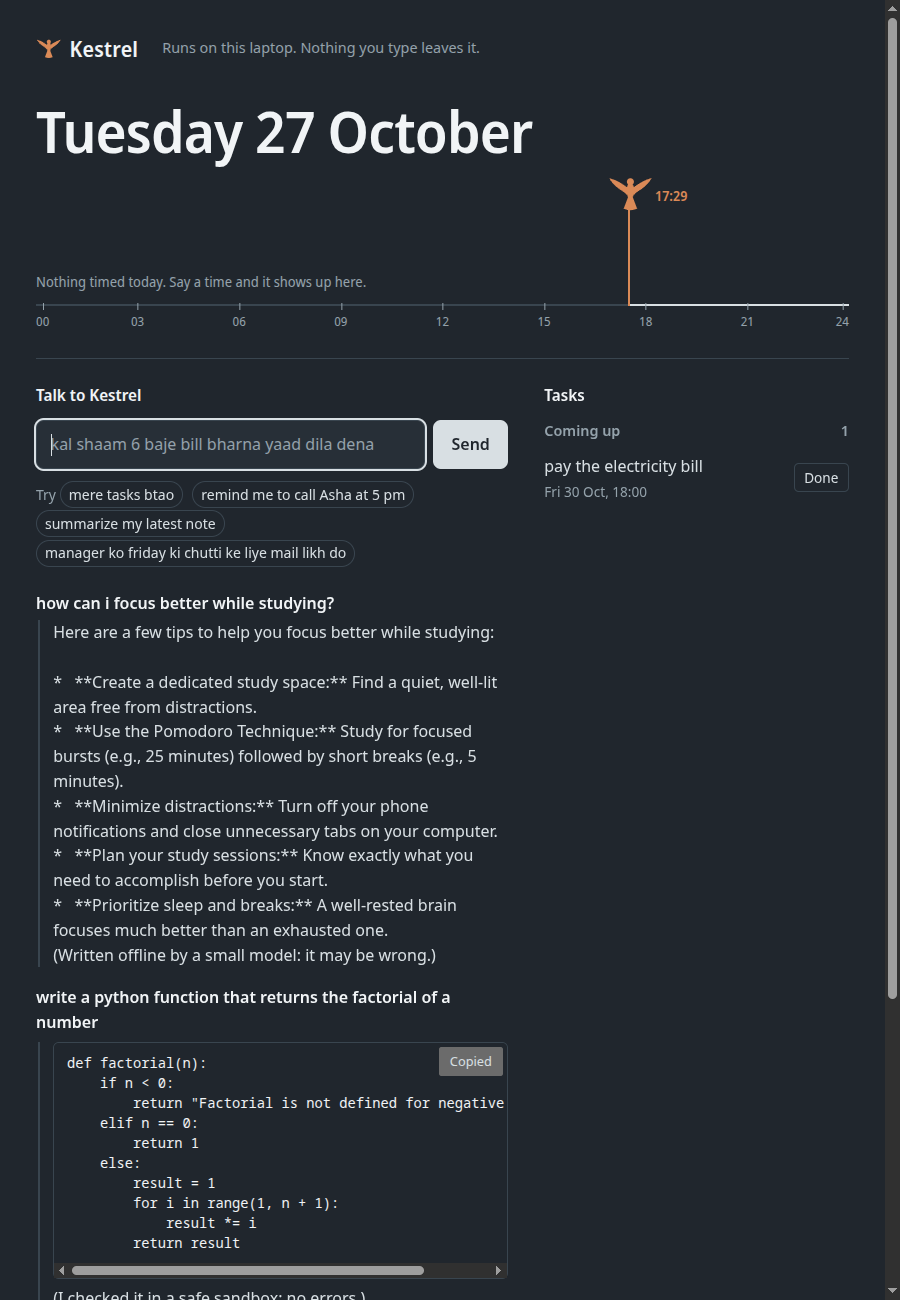
\includegraphics[width=0.62\textwidth]{../../experiments/logs/v3/acceptance/page_headed.png}
\caption{Kestrel's browser page during the acceptance run (headed Chrome on the author's screen): the day strip with
the kestrel marking the current time, the request box with example requests, the task list, a chat answer with its
caveat, and a code answer in a code box with a Copy button and the sandbox's check below it.}
\label{fig:page}
\end{figure}

The examples below are real requests and answers from the acceptance run (Section~\ref{sec:acceptance}), copied from
its log. That run used a scratch copy of the service with sample notes, not the author's own notes.

\paragraph{Tasks and reminders.} \req{kal shaam 6 baje bill bharna yaad dila dena} $\to$ \ans{created task \#2: bill
bharna (due 2026-10-28 18:00)}. \req{move task 2 to friday} $\to$ \ans{task \#2 now due 2026-10-30}. Deleting asks
first. A timed task pops up as a desktop notification at its time.

\paragraph{Notes by meaning.} The keyword search still runs first. When it finds fewer than three notes, the note closest
in meaning is added if it is close enough: \req{search my notes for maa ke liye tohfa} $\to$ \ans{found 1 note: -
2026-09-08-mom-birthday.md (by meaning)}, although the keyword search, which needs every word of the query in a note,
found nothing.

\paragraph{Questions answered from the notes.} \req{maa ka birthday kab hai?} $\to$ \ans{Maa ka birthday 20 September
hai. (from 2026-09-08-mom-birthday.md)}. When the notes do not say: \req{goa wale hotel ka naam kya hai?} $\to$
\ans{The notes do not say this: so the reply is not available for this information}. An answer is shown only if every
number and name in it occurs in the notes.

\paragraph{Emails, rewriting and translation.} \req{manager ko friday ki chutti ke liye mail likh do} $\to$ a Hinglish
draft starting \ans{Subject: Friday ki chutti ke liye request}. \req{make this polite: send me the file now} $\to$
\ans{Could you please send me the file now?} \req{translate to english: aaj bahut garmi hai} $\to$ \ans{It is very hot
today}. Translation into Hindi is written in Devanagari script; Hinglish stays in Latin letters, although a
request to translate into Hinglish often came back in English (\kv{writer.final.translate-hinglish} on development
items).

\paragraph{Chat.} General questions, explanations, ideas and poems are answered by the language model, and every such
answer ends with \ans{(Written offline by a small model: it may be wrong.)}. Questions that need live data or the
internet (\req{what's the weather in delhi today?}) are refused.

\paragraph{Code.} \req{fix this function: def add(a, b): return a - b} $\to$ the fixed function, then \ans{(I checked it
in a safe sandbox: no errors.)} and \ans{(Written offline by a small model: try it before you rely on it.)}. On the page,
code appears in a box with a Copy button.

\paragraph{Saving to notes.} \req{Buy rice, dal and oil on Saturday from the market. add this to notes} asks
\ans{Save this as a new note, 2026-10-27-buy-rice-dal-and-oil-on-saturday-from.md (10 words)?} and, after a yes, saves
the text exactly as typed. It never writes over an existing file.

\paragraph{Where to use it.} In the browser page (Figure~\ref{fig:page}), opened with \texttt{kestrel open} or from the
applications menu, or in a terminal with \texttt{kestrel chat} and \texttt{kestrel say}. Answers from the language model
appear as they are written, except answers from the notes and note summaries, which appear once they have been checked.

% ---------------------------------------------------------------------------------------------------------------
\section{How it works}\label{sec:how}

\begin{figure}[t]
\centering
% The v3 request path (Figure 1 of the paper, Figure 2 of the report); no numbers.
\resizebox{\textwidth}{!}{%
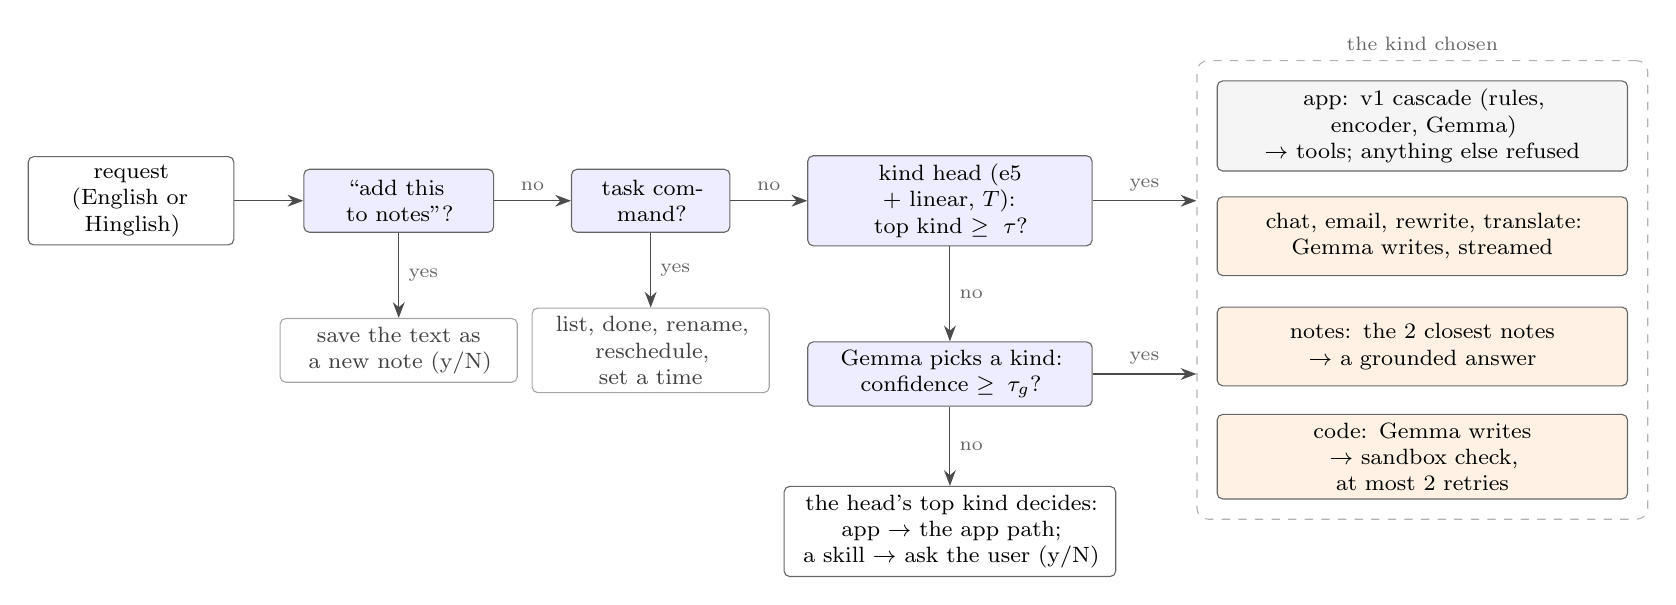
\begin{tikzpicture}[
  font=\footnotesize,
  box/.style={draw=black!60, rounded corners=2pt, align=center, inner sep=3pt, minimum height=8mm},
  act/.style={box, draw=black!35, text=black!75, text width=28mm},
  dec/.style={box, fill=blue!7},
  dest/.style={box, fill=orange!10, text width=50mm, minimum height=10mm},
  arr/.style={-{Stealth[length=2mm]}, black!70},
  lab/.style={font=\scriptsize, text=black!60}]
  \node[box, text width=24mm] (req) at (0,0) {request\\(English or Hinglish)};
  \node[dec, text width=22mm] (save) at (3.4,0) {``add this to notes''?};
  \node[dec, text width=18mm] (cmd) at (6.6,0) {task command?};
  \node[dec, text width=34mm] (head) at (10.4,0) {kind head (e5 + linear, $T$):\\top kind $\ge\tau$?};
  \node[dec, text width=34mm] (gem) at (10.4,-2.2) {Gemma picks a kind:\\confidence $\ge\tau_g$?};
  \node[box, text width=40mm] (last) at (10.4,-4.2) {the head's top kind decides:\\app $\to$ the app path;\\a skill $\to$ ask the user (y/N)};
  \node[act] (saveact) at (3.4,-1.9) {save the text as\\a new note (y/N)};
  \node[act] (cmdact) at (6.6,-1.9) {list, done, rename,\\reschedule, set a time};
  \node[dest, fill=black!4] (app) at (16.4,0.95) {app: v1 cascade (rules, encoder, Gemma)\\$\to$ tools; anything else refused};
  \node[dest] (w) at (16.4,-0.45) {chat, email, rewrite, translate:\\Gemma writes, streamed};
  \node[dest] (qa) at (16.4,-1.85) {notes: the 2 closest notes\\$\to$ a grounded answer};
  \node[dest] (code) at (16.4,-3.25) {code: Gemma writes $\to$ sandbox check,\\at most 2 retries};
  \node[draw=black!30, dashed, rounded corners, fit=(app)(w)(qa)(code), inner sep=2.5mm,
        label={[lab]above:the kind chosen}] (dests) {};
  \draw[arr] (req) -- (save);
  \draw[arr] (save) -- node[lab, above]{no} (cmd);
  \draw[arr] (cmd) -- node[lab, above]{no} (head);
  \draw[arr] (save) -- node[lab, right]{yes} (saveact);
  \draw[arr] (cmd) -- node[lab, right]{yes} (cmdact);
  \draw[arr] (head) -- node[lab, right]{no} (gem);
  \draw[arr] (gem) -- node[lab, right]{no} (last);
  \draw[arr] (head.east) -- node[lab, above]{yes} (head.east -| dests.west);
  \draw[arr] (gem.east) -- node[lab, above]{yes} (gem.east -| dests.west);
\end{tikzpicture}}

\caption{The path of a request. Saving a note and task commands are recognised first. Then a small, fast classifier
decides the kind of answer: the old app path, or one of the new skills. When it is unsure, the language model decides;
when that is unsure too, Kestrel proposes a skill as a yes/no question, or takes the old path if the request leans to
the app.}
\label{fig:arch}
\end{figure}

\subsection{The service}
One program, \texttt{kestrel serve}, runs from login and keeps the cheap parts loaded: keyword rules and the sentence
encoder (multilingual-e5-small). The language model, Gemma-4-E2B at 4-bit, runs in a separate worker process that starts
on the first request that needs it and stops after 10 idle minutes, which gives its memory back. The terminal client and
the browser page talk to the service over a local socket and a local web server on 127.0.0.1 that needs a key.

\subsection{Deciding the kind of answer}
Every request that is not a task command first gets a \emph{kind}: \emph{app} (the v1/v2 path: tasks, notes search and
summaries, memory, small talk, refusals), \emph{chat}, \emph{email}, \emph{rewrite}, \emph{translate}, \emph{notes} (a
question about the user's own life) or \emph{code}. The encoder turns the request into a vector, and a small trained
classifier on top gives a probability for each kind. Its probabilities are calibrated (temperature scaling): fitted so
that its confidence stays close to how often it is right on held-out data. Then:
\begin{enumerate}
  \item if the top kind reaches the threshold $\tau=\kv{fb2.tau}$, it decides;
  \item otherwise Gemma reads the request with a short description of each kind and chooses one; if its calibrated
  confidence reaches $\tau_g=\kv{fb2.taug}$, its choice decides (about \kv{fb2.ms.p50}\ms\ on this laptop);
  \item otherwise, if the classifier's top kind is a skill, Kestrel asks, for example \ans{Write this as an email or
  message draft?}; if it is app, the request takes the old path.
\end{enumerate}
The thresholds were chosen on development data by a rule written down before the run: fewest wrong decisions, then
fewest questions to the user.

\subsection{Notes by meaning and answers from notes}
Each note is cut into chunks (its title and one paragraph), and each chunk becomes a vector once; the vectors are cached
and recomputed only for notes that change. A search query becomes a vector too, and the closest note is added if it is
close enough (cosine similarity at least $\theta=\kv{mtt.theta}$). The encoder does not understand Romanized Hindi well,
so a query with common Hindi words is first put into English by Gemma (\req{maa ke liye tohfa} became \req{gift for
mother}). For a notes question, the two closest notes go to Gemma with the instruction to answer only from them, in the
question's language, or to say exactly \texttt{NOT IN NOTES}. A grounding check then rejects an answer whose numbers or
names are not in the notes.

\subsection{Code in a sandbox}
For a code request Gemma writes standard-library Python. The code then runs inside bubblewrap, a Linux sandbox: no
network, no access to the home folder, a read-only system, an empty temporary folder, and limits of 512~MiB of memory,
10~s of processor time, 10~MiB files and 64 processes. Code is imported (so it compiles and its top level runs); code
that waits for input is only compiled, since the sandbox cannot type for it. A syntax error, a crash or a timeout is sent
back to Gemma, at most twice, with the error. The answer always says what was checked.

\subsection{Two changes that made the service fast to start}
\begin{itemize}
  \item \textbf{Memory-mapped weights.} The model file is mapped into memory instead of copied. The memory the system
  cannot take back fell from \kv{mmap.copy.cold.anon} to \kv{mmap.map.cold.anon}\MiB\ (\kv{mmap.anon.cut} less), and
  loading became faster (\kv{mmap.copy.cold.load} to \kv{mmap.map.cold.load}\ms\ from a cold disk cache).
  \item \textbf{A saved prompt.} Before answering, the worker reads a \kv{worker.prefix.tokens}-token prompt of
  examples. v3 saves the model's state after reading it and loads that state next time. The worker became ready in
  \kv{worker.hit.s}\s\ instead of \kv{worker.v2.s}\s\ (medians of \kv{worker.v2.n} starts).
\end{itemize}

\begin{figure}[t]
\centering
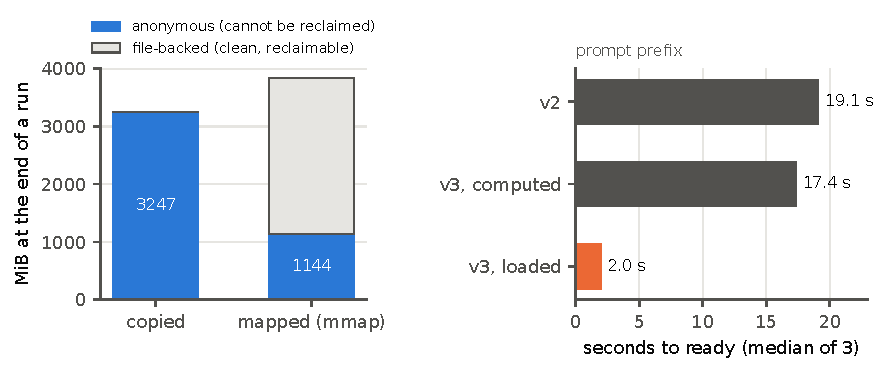
\includegraphics[width=\textwidth]{figures/memory.pdf}
\caption{Left: memory at the end of a run with the model's weights copied or mapped; the grey part is the mapped file,
which the system can drop when it needs memory. Right: seconds until the language model's worker is ready.}
\label{fig:memory}
\end{figure}

% ---------------------------------------------------------------------------------------------------------------
\section{How it was built}

\paragraph{Decisions on record.} Every design choice of v3 was recorded as a decision with its context, the options
considered and the reason (thirteen records, from the goal on 26 October 2026 to the freeze on 27 October 2026;
Appendix~\ref{app:decisions}). The author made each decision, mostly by accepting a stated recommendation.

\paragraph{Technology.} The assistant is written in Rust (a workspace of crates; the v3 parts live in the command-line
app, and the memory-mapped load and the saved prompt in the inference crate), and runs the models through llama.cpp. Evaluation scripts are Python. The sandbox is bubblewrap, and the browser
page is a single self-contained HTML page served by Kestrel itself, tested with Google Chrome over its DevTools protocol.
No paid service was used, and only models already on the laptop were used.

\paragraph{Data and fair testing.} Each part was measured on a small evaluation set written for it
(Table~\ref{tab:data}), in English and Hinglish pairs, grouped into \emph{families} of similar requests. Each set was
split by family into development data, used to choose every setting, and a test split, run once at the end. Most sets
were reviewed card by card by the author on a review page; for the code set and the third kinds set the author waived the
review, and they were reviewed by the AI assistant that drafted them, with a separate agent checking the files against
written criteria.

\begin{table}[h]
\centering\small
\caption{Evaluation sets. All are synthetic and split by family.}
\label{tab:data}
\resizebox{\textwidth}{!}{% Generated by experiments/analysis/paper_assets_v3.py.
\begin{tabular}{llll}
\toprule
Dataset & Labels / content & Items (train / cal / val / test) & Review \\
\midrule
Kestrel-Kinds-v1 & 6 kinds & 920 / 115 / 136 / 256 & reviewed \\
Kestrel-Kinds-v2 & 7 kinds (+ code) & 1000 / 123 / 152 / 280 (24 fresh) & claude reviewed \\
Kestrel-NotesQ-v0 & 18 fixture notes & dev 22 (4 none) / test 20 (2 none) & reviewed \\
Kestrel-NotesQA-v0 & same notes & dev 26 (6 unans.) / test 25 (6 unans.) & reviewed \\
Kestrel-CodeTasks-v0 & 4 types & dev 24 / test 24 (24 families) & claude reviewed \\
\bottomrule
\end{tabular}
}
\end{table}

% ---------------------------------------------------------------------------------------------------------------
\section{Results}\label{sec:results}

\subsection{Choosing the kind of answer}
On Kinds-v2's test split, \kv{kt2.hg.right} decisions were right (\kv{kt2.hg.right.pct}); \kv{kt2.hg.asked} requests were
asked about, \kv{kt2.hg.sentoldway} skill requests were sent the old way (the app path), and \kv{kt2.hg.notaskedfor} times a
skill was started that the request did not ask for: three jokes and a web search answered as chat, a time question sent
to notes, and a loop fix sent to rewrite. English and Hinglish were close (\kv{kt2.hg.en} and \kv{kt2.hg.hi}). Without the
language model's second opinion, only \kv{kt2.ha.right} were right: more requests were asked about (\kv{kt2.ha.asked}) or sent the old way
(\kv{kt2.ha.sentoldway}).

\kv{kv1.test} of these \kv{kt2.n} test requests had already been used once, to test the previous version of the kinds
set, and the new training families were written after its mistakes were known; so this result is optimistic. On the
\kv{kv2.test.fresh} fresh requests, \kv{kt2.fresh.hg.right} were right. Per kind (Table~\ref{tab:perkind}), chat and
translation were always recognised, code \kv{kt2.hg.kind.code}, email \kv{kt2.hg.kind.email} and notes questions
\kv{kt2.hg.kind.notes}; rewrite requests only \kv{kt2.hg.kind.rewrite}, most of the rest being asked about first.

\begin{table}[h]
\centering\small
\caption{Right decisions per kind on the two test splits. Kinds-v1 had no code kind.}
\label{tab:perkind}
% Generated by experiments/analysis/paper_assets_v3.py.
\begin{tabular}{lrrrr}
\toprule
 & \multicolumn{2}{c}{Kinds-v1 test} & \multicolumn{2}{c}{Kinds-v2 test} \\
\cmidrule(lr){2-3}\cmidrule(lr){4-5}
Gold kind & head alone & head + Gemma & head alone & head + Gemma \\
\midrule
app & 179/180 & 180/180 & 181/184 & 178/184 \\
chat & 2/16 & 11/16 & 6/20 & 20/20 \\
code & -- & -- & 1/8 & 7/8 \\
email & 12/16 & 13/16 & 12/16 & 15/16 \\
notes & 1/12 & 1/12 & 7/16 & 12/16 \\
rewrite & 3/16 & 4/16 & 6/20 & 8/20 \\
translate & 9/16 & 11/16 & 8/16 & 16/16 \\
\bottomrule
\end{tabular}

\end{table}

\begin{figure}[h]
\centering
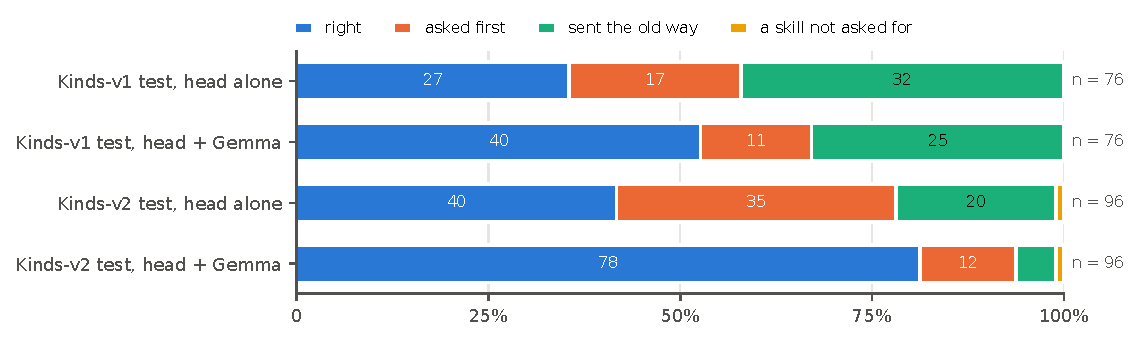
\includegraphics[width=\textwidth]{figures/kinds.pdf}
\caption{What happened to requests for a skill on the test splits, with the classifier alone and with the language
model's second opinion.}
\label{fig:kinds}
\end{figure}

\subsection{Finding notes by meaning}
Every query in this set misses its note by keywords, so every find is the meaning search's. Before the translation step,
only \kv{md.found.hi} Hinglish development queries found their note; with it, \kv{mdt.found.hi}. On the test split the
right note was added for \kv{mtt.found} queries (\kv{mtt.found.en} English, \kv{mtt.found.hi} Hinglish), and no note was
added to the \kv{notesq.test.none} queries that have none. In two of the misses the right note was the closest but just
below the threshold, so nothing was added; for \req{festival shopping} (in both languages) the closest note was the Goa trip
note, also below the threshold, so nothing was added either.

\subsection{Answering from the notes}
On the test split, all \kv{qa.test.ans} answerable questions were answered with the right facts, and all
\kv{qa.test.un} unanswerable ones got the ``not in your notes'' reply; generating an answer took \kv{qa.test.s.mean}\s\ on average.
On development data \kv{qa.dev.un} unanswerable questions were declined: twice the model said in its own words that the
notes do not give a cake's price, instead of the exact marker. The language of the answer is weaker than its content:
in the test run (before a fix), \kv{qa.test.hinglish} answers to Hinglish questions were Hinglish; with the fix,
\kv{qa.dev.hinglish} on development data.

\subsection{Code}
Three models already on the laptop were compared on development data. After the checks were reviewed, Gemma-4-E2B and
Qwen3-4B were both right \kv{code.resc.gemma} times, but Gemma's generation took \kv{code.resc.gemma.s}\s\ per request against
\kv{code.resc.qbig.s}\s\ and needs no second model in memory, so Gemma does code too. On the test split, run once, Gemma
was right \kv{code.test.all} times: every function, fix and explanation, but only \kv{code.test.script} scripts. The failed
scripts kept reading input until the input ended (and crashed), stopped at the first empty line, or reversed the letters
of a line instead of its words. Generation took \kv{code.test.s}\s\ per request on average. The sandbox found no error in any answer, so
the retry loop never ran. Two weaknesses that the scores do not show: the three English requests to explain code were
answered in Hinglish, and one explanation stated a wrong output and still passed, because explanations are judged by
the facts they must contain.

\begin{table}[h]
\centering\small
\caption{Code requests right, by type (6 per type), and generation seconds per request.}
\label{tab:code}
\resizebox{\textwidth}{!}{% Generated by experiments/analysis/paper_assets_v3.py.
\begin{tabular}{lrrrrrr}
\toprule
Model and run & function & script & fix & explain & all & gen.\ s / request \\
\midrule
Gemma-4-E2B, first harness and checks (dev) & 6/6 & 1/6 & 6/6 & 6/6 & 19/24 & 11.1 \\
Qwen3-1.7B, first harness and checks (dev) & 5/6 & 1/6 & 5/6 & 6/6 & 17/24 & 10.4 \\
Qwen3-4B, first harness and checks (dev) & 6/6 & 5/6 & 6/6 & 6/6 & 23/24 & 29.0 \\
\midrule
Gemma-4-E2B, final harness (dev) & 6/6 & 5/6 & 6/6 & 6/6 & 23/24 & 9.1 \\
Gemma-4-E2B, final harness (\textbf{test}, once) & 6/6 & 3/6 & 6/6 & 6/6 & 21/24 & 8.9 \\
\bottomrule
\end{tabular}
}
\end{table}

\subsection{Acceptance run}\label{sec:acceptance}
Before the freeze, every goal feature was used end to end on a scratch copy of the service with sample notes: the same
requests a user would type, over the same socket the terminal client uses, with yes/no questions answered.
\kv{acc.socket} requests passed. The browser page was driven step by step in Chrome, headless and in a visible window,
and passed \kv{acc.page.headless} and \kv{acc.page.headed} steps (load, a Try button, a task made and listed, the page's
own yes/no question, a code box, the Copy button read back from the clipboard, a streamed chat answer with its caveat).
A reminder due at \kv{acc.reminder.due} popped up at \kv{acc.reminder.rang}. The automated tests passed: \kv{acc.cargo}
Rust tests, \kv{acc.pytest} Python tests, \kv{acc.bwrap} sandbox tests and \kv{acc.worker} model-worker tests.

The two failed requests: \req{how much is my rent?} was refused, because both the classifier and Gemma took it for an
app request (asked as a notes question, the same answer component gets it right); and \req{which preferences have i
set?} found nothing, because the memory search matches the stored words.

\begin{table}[h]
\centering\small
\caption{Seconds until the whole answer, from the acceptance run: one run on the laptop as found, not a
benchmark.}
\label{tab:times}
\begin{tabular}{lr@{\hspace{2.2em}}lr}
\toprule
Request & s & Request & s \\
\midrule
add a task with a time & \kv{acc.s.task} & translate into Hindi & \kv{acc.s.tohindi} \\
add a task, Hinglish & \kv{acc.s.taskhi} & translate into English & \kv{acc.s.toenglish} \\
keyword search & \kv{acc.s.search} & rewrite politely & \kv{acc.s.rewrite} \\
search by meaning & \kv{acc.s.meaning} & email (Hinglish / English) & \kv{acc.s.emailhi} / \kv{acc.s.email} \\
search by meaning, Hinglish & \kv{acc.s.meaninghi} & answer from notes & \kv{acc.s.qa} \\
summary of a note & \kv{acc.s.summary} & write a function & \kv{acc.s.codefn} \\
chat: a short poem & \kv{acc.s.poem} & fix a function & \kv{acc.s.codefix} \\
chat: an explanation & \kv{acc.s.chat} & a very long essay (cut off) & \kv{acc.s.essay} \\
\bottomrule
\end{tabular}
\end{table}

% ---------------------------------------------------------------------------------------------------------------
\section{Known limitations}\label{sec:limits}

These \kv{acc.limits} were written down at the freeze and not fixed, because the author froze the product:
\begin{enumerate}
  \item Some notes questions are refused (\req{how much is my rent?}); others are answered (\req{maa ka birthday kab hai?}).
  \item \req{which preferences have i set?} finds nothing, although a preference is stored.
  \item \req{write a program to solve X} goes to chat: the whole program comes, but without the sandbox check.
  \item Rewrite requests are often asked about first.
  \item Scripts that read input to its end are Gemma's weak spot.
  \item Jokes are answered by chat; \req{what time is it in London} goes to notes.
  \item Markdown in chat answers (bold, bullets) is shown as typed.
  \item Answers from notes to Hinglish questions are sometimes English.
  \item Code may use Python's standard library only, and is checked by import or compile, never run with input.
  \item Once, code did not show on the author's page; this could not be reproduced.
  \item The page can be shared on the wifi over plain HTTP when the service is installed that way (off now).
  \item There is no memory of the conversation: \req{continue} or a follow-up does not see the last answer.
\end{enumerate}
In addition, every evaluation set is small and synthetic, about an imagined user's life; real use will find other
mistakes. Energy use was not measured.

% ---------------------------------------------------------------------------------------------------------------
\section{Installing and using it}

Setup follows the repository's README: a Python environment, the models fetched and checked, the encoder converted,
the heads trained (for v3 also the kind head, \texttt{python experiments/v3/kind\_head.py -{}-dataset kinds\_v2}), and a
release build with the \texttt{llama} feature. Then:
\begin{itemize}
  \item \texttt{scripts/install\_service.sh \textasciitilde/notes} installs the always-on service for a notes folder;
  \texttt{scripts/install\_reminders.sh} adds the morning reminder.
  \item \texttt{kestrel open} opens the page; \texttt{kestrel chat} starts a conversation in a terminal;
  \texttt{kestrel say "mere tasks btao"} sends one request; \texttt{kestrel stop} frees all of its memory.
\end{itemize}
The installed v3 service runs from its own checkout (a git worktree) at the tested build, commit \texttt{86cb3a7},
so the research can switch branches in the main checkout without touching it.

% ---------------------------------------------------------------------------------------------------------------
\section{What comes next}

\begin{itemize}
  \item \textbf{Learn from real mistakes.} The next round starts from the author's own misrouted requests: new kinds and
  code sets built from them, reviewed, with a fresh test split.
  \item \textbf{A bigger machine (v4).} Larger models need more memory and speed than this laptop has; on it, Qwen3-4B
  already writes only \kv{e0.qbig.tg} tokens per second.
  \item \textbf{The research first.} From the week of 1 November 2026 the pre-registered research (personalization and
  quantization experiments, final statistics) continues; heavy runs of the two never overlap.
\end{itemize}

\appendix
% ---------------------------------------------------------------------------------------------------------------
\section{Decision record}\label{app:decisions}

\begin{small}
\begin{tabularx}{\textwidth}{@{}lX@{}}
\toprule
Decision & What was decided \\
\midrule
ADR-036 & v3's goal on this laptop, fully offline; v4 is a bigger machine. \\
ADR-037 & A kind decision before the research cascade; the first kinds data set. \\
ADR-038 & Chat answers timeless explanations with a visible caveat; more families before review. \\
ADR-039 & Notes found by meaning after the keyword search, in the app only. \\
ADR-040 & Hinglish queries go through English; only the closest note is added. \\
ADR-041 & Notes Q\&A: a \emph{notes} kind; answers only from the notes, grounded, with ``not in your notes''. \\
ADR-042 & After the notes review: freeze the notes sets, test once on Kinds-v1, more notes families. \\
ADR-043 & v3 becomes the always-on service, run from its own worktree. \\
ADR-044 & Qwen3-4B for code (superseded by ADR-046); the code loop retries only on the sandbox's own errors; one
review for the code and Kinds-v2 sets. \\
ADR-045 & The author waives that review; the AI assistant reviews with an independent agent. \\
ADR-046 & Gemma writes and fixes code too (one model in the service). \\
ADR-047 & The page may be shared on the wifi (off by default). \\
ADR-048 & v3 frozen after the acceptance run (tag \texttt{v3-frozen}). \\
\bottomrule
\end{tabularx}
\end{small}

\section{Where the numbers come from}
Every measured value, share and table entry in this report comes from the committed logs through the script
\path{experiments/analysis/paper_assets_v3.py}; its tests fail if a document asks for a value the script does not
generate. Configuration constants (sandbox limits, retries, the number of notes given) and a few small counts in the
prose (such as the misrouted requests named in Section~\ref{sec:results}) are typed and were checked by hand. The logs are under \texttt{experiments/logs/v3/}: \texttt{kinds/}, \texttt{notes/}, \texttt{code/},
\texttt{writer/}, \texttt{mmap/}, \texttt{worker/} and \texttt{acceptance/}; the laptop's description is in
\path{experiments/PREREG.md} and its model speeds in \path{experiments/logs/E0/}. \path{paper/v3/number_check.md} records an
independent check of every number.

\end{document}
